\documentclass[a4paper,10pt,notitlepage]{report}
\usepackage[utf8]{inputenc}
\usepackage{authblk}
\usepackage{geometry}
\usepackage{graphicx}
\usepackage{tabulary}
\usepackage{amsmath}
\usepackage{mathtools}
\usepackage{float}
\usepackage{cite}
\usepackage{color}
\usepackage{caption}
\usepackage{subcaption}
% \usepackage[pdfborder={0 0 0.6}]{hyperref}
\usepackage{hyperref}
\usepackage{enumitem}
\usepackage{multirow}
\usepackage{multicol}
\usepackage{makecell}
\usepackage{bm}
\usepackage{wrapfig}

%%%%%%%%%%%%%%%%%%%%%%%%%%%%%%%%%%%%%%% making figures in the subsection where placed (according to https://tex.stackexchange.com/questions/279/how-do-i-ensure-that-figures-appear-in-the-section-theyre-associated-with/235312#235312 )
\usepackage{placeins}

\let\Oldsection\section
\renewcommand{\section}{\FloatBarrier\Oldsection}

\let\Oldsubsection\subsection
\renewcommand{\subsection}{\FloatBarrier\Oldsubsection}

\let\Oldsubsubsection\subsubsection
\renewcommand{\subsubsection}{\FloatBarrier\Oldsubsubsection}
%%%%%%%%%%%%%%%%%%%%%%%%%%%%%%%%%%%%%%%5

\pdfinfo{%
  /Title    ()
  /Author   (Leszek Adamczyk, Łukasz Fulek, Rafał Sikora)
}


%colors
\definecolor{gray}{rgb}{0.5, 0.5, 0.5}

%additional symbols
\newcommand{\Pom}{\texorpdfstring{I$\!$P}{P}}             % gives pomeron symbol
\newcommand{\Reg}{\texorpdfstring{I$\!$R}{R}}               % gives pomeron symbol
\newcommand{\DPE}{D\Pom E}
\newcommand{\Pomeron}{\Pom omeron}
\newcommand{\Reggeon}{\Reg eggeon}

% ---- ---- additional commands ---- ----
\newcommand{\specialcell}[2][c]{%
  \begin{tabular}[#1]{@{}c@{}}#2\end{tabular}}

\makeatletter
\def\tagform@#1{\maketag@@@{(\ignorespaces#1\unskip\@@italiccorr)}}
\renewcommand{\eqref}[1]{\textup{{\normalfont(\ref{#1}}\normalfont)}}
\makeatother
  
\makeatletter
\newcommand{\Spvek}[2][l]{%
  \gdef\@VORNE{1}
  \left[\hskip-\arraycolsep%
    \begin{array}{#1}\vekSp@lten{#2}\end{array}%
  \hskip-\arraycolsep\right]}
\def\vekSp@lten#1{\xvekSp@lten#1;vekL@stLine;}
\def\vekL@stLine{vekL@stLine}
\def\xvekSp@lten#1;{\def\temp{#1}%
  \ifx\temp\vekL@stLine
  \else
    \ifnum\@VORNE=1\gdef\@VORNE{0}
    \else\@arraycr\fi%
    #1%
    \expandafter\xvekSp@lten
  \fi}
\makeatother
% ---- ---- ---- ---- ---- ---- ---- ----

%chapter heading
\makeatletter
\renewcommand{\@makechapterhead}[1]{%
 \vspace*{-18\p@}%
  {\parindent \z@ \raggedright
%     \LARGE \bfseries \thechapter. #1\par\nobreak
%     \vskip 40\p@
      \Huge \bfseries \thechapter. #1\par\nobreak
      \vskip 20\p@
  }}
\makeatother


% Title Page
\title{\textbf{Supplementary note on diffractive analyses\\of 2015 proton-proton data:\\[20pt]\large{\cite{AnalysisNoteRafal}~Measurement of Central Exclusive Production of $\bm{h\bar{h}}$ pairs ($\bm{h=\pi,K,p}$) with Roman Pot detectors in diffractive\\proton-proton interactions at~$\bm{\sqrt{s}=}$~200~GeV\\[10pt]\cite{AnalysisNoteLukasz}~Measurement of particle production with Roman Pot detectors\\in diffractive proton-proton interactions at~$\bm{\sqrt{s}=}$~200~GeV\\}}\vspace*{10pt}}
\author[1]{\href{mailto:leszek.adamczyk@agh.edu.pl}{Leszek Adamczyk}}
\author[1]{\href{mailto:lukasz.fulek@fis.agh.edu.pl}{Łukasz Fulek}}
\author[1]{\href{mailto:rafal.sikora@fis.agh.edu.pl}{Rafał Sikora}}
\affil[1]{AGH University of Science and Technology, FPACS, Kraków, Poland}


\setcounter{Maxaffil}{0}
\renewcommand\Affilfont{\itshape\small}
\renewcommand{\bibname}{References}

\begin{document}

\begin{center}
\begin{minipage}[c]{0.12\linewidth}%
\vspace{5.5pt}\textbf{\LARGE{of the}}
\end{minipage}
\begin{minipage}[c]{0.15\linewidth}%
\hspace*{-8pt}
\includegraphics[width=\linewidth]{graphics/STAR_logo.pdf}
\end{minipage}~
\begin{minipage}[c]{0.24\linewidth}%
\vspace{9pt}\hspace*{-8pt}\textbf{\LARGE{Experiment}}
\end{minipage}\\[-50pt]
\textbf{\LARGE{Analysis Note}}

\vspace*{125pt}
\begin{minipage}{\linewidth}
\maketitle
\begin{abstract}
In this note we present supplementary material related to analyses of diffractive processes based on 2015 data from proton-proton collisions at $\sqrt{s}=200$~GeV. This dataset was collected with newly installed Roman Pot detectors in Phase II* configuration which ensured efficient triggering and measuring diffractively scattered protons.\\\indent We focus on calculation of efficiencies, corrections to Monte Carlo simulations and derivation of systematic uncertainties of our measurements.
\end{abstract}
\thispagestyle{empty}
\end{minipage}

% \vspace{50pt}

%  \Huge{\textbf{\textit{DRAFT}}}
\end{center}


\clearpage
\thispagestyle{empty}
\newgeometry{hmargin={2cm, 2cm}, height=10.0in}

\setcounter{secnumdepth}{3}
\setcounter{tocdepth}{4}
\tableofcontents


 
%% =====  EFFICIENCIES ====
%%===========================================================%%
%%                                                           %%
%%                       EFFICIENCIES                        %%
%%                                                           %%
%%===========================================================%%


\chapter{Efficiencies}\label{chap:efficiencies}
\section{General overview}\label{sec:effGeneralOverview}
It is the best to apply the corrections to the measured distributions  that are based on real data analysis. However, due to the complexity of the processes we are studying, it is necessary to obtain corrections from the MC simulation. Whenever possible, we compare efficiencies obtained from data with those from the MC and introduce appropriate corrections to the MC if necessary.

It is prefered to get the detector to true-level corrections from the MC, which is dedicated to the studied physics process. However, for this purpose, the~statistics in the MC should be several times greater (preferably an order of magnitude) than we have in the data for analysis. This is not possible with generally low total efficiency $\left(\textrm{TPC \& TOF \& RP}\right)$. On the other hand, such efficiencies depend on the modeling of the studied process and require a good description of all generally multidimensional distributions  by MC. Since that, the basic method of corrections that we use in the analyses is the method of factorization of global efficiency into the product of single-particle efficiencies (separate for each central particle and forward protons). Thereby,  statistically precise multidimensional corrections on TPC, TOF and RP are obtained. Nevertheless, this method does not correct on the migration effects caused by the finite detector resolution and is sensitive to the binning. Whenever possible, we use both methods of correction (at least in the consistency tests for MC samples). In this note, only the single-particle corrections are described, which are common for both analyses.

\section{TPC track acceptance and reconstruction efficiency}\label{sec:tpcAccAndEff}
We defined joint acceptance and efficiency of reconstruction of a track in the TPC, $\epsilon_{\textrm{\tiny TPC}}$, as the probability that particle from the primary interaction generates signal in the detector which is reconstructed as a global track that satisfies all quality criteria (cuts~\ref{sec:TpcQualityCuts}).
To derive this quantity the single particle STARsim MC embedded into zero-bias trigger data taken simultaneously with physics triggers 
 was used.
\subsection{STAR nominal method}
Technically, the common method used by the STAR to obtain  $\epsilon_{\textrm{\tiny TPC}}$ is the following procedure:
\begin{enumerate}
	\item True-level primary particles of given ID and charge were selected ($set~A$).
	\item Each particle from $set~A$ was checked if at least one global TPC track with more than half of hit points associated to it was generated by true-level particle  (definition of true level particle-track matching, idTruth from StMuTrack collection). All particles from $set~A$ which have associated global track satisfying quality criteria (cut~\ref{sec:TpcQualityCuts}) formed $set~B$.
	\item The joint TPC acceptance and efficiency was calculated as the ratio of the histograms of true level quantities (such as $p_{T}$, $\eta$, $z_{\textrm{vtx}}$) for particles from $set~B$ and particles from $set~A$:
	\begin{equation}\label{eq:tpcAccAndEffDefinition}
	\epsilon_{\textrm{\tiny TPC}}\left(p_{T}, \eta, z_{vtx};~\textrm{sign},\textrm{PID}\right) = \frac{(p_{T},\eta, z_{vtx})~\textrm{histogram for particles of given sign and ID from}~set~B}{(p_{T},\eta, z_{vtx})~\textrm{histogram for particles of given sign and ID from}~set~A}.
	\end{equation}
	
\end{enumerate}
\subsubsection{Global track to true level particle matching}
It was found during the analysis that in about $1\%$ events there are more than one reconstructed global track matched with the same true level particle, which is shown in Fig.~\ref{fig:trackSplittingNominal}, separatelly for true level pions, kaons and protons.
\begin{figure}[ht]
	\centering
	\parbox{0.329\textwidth}{
		\centering
		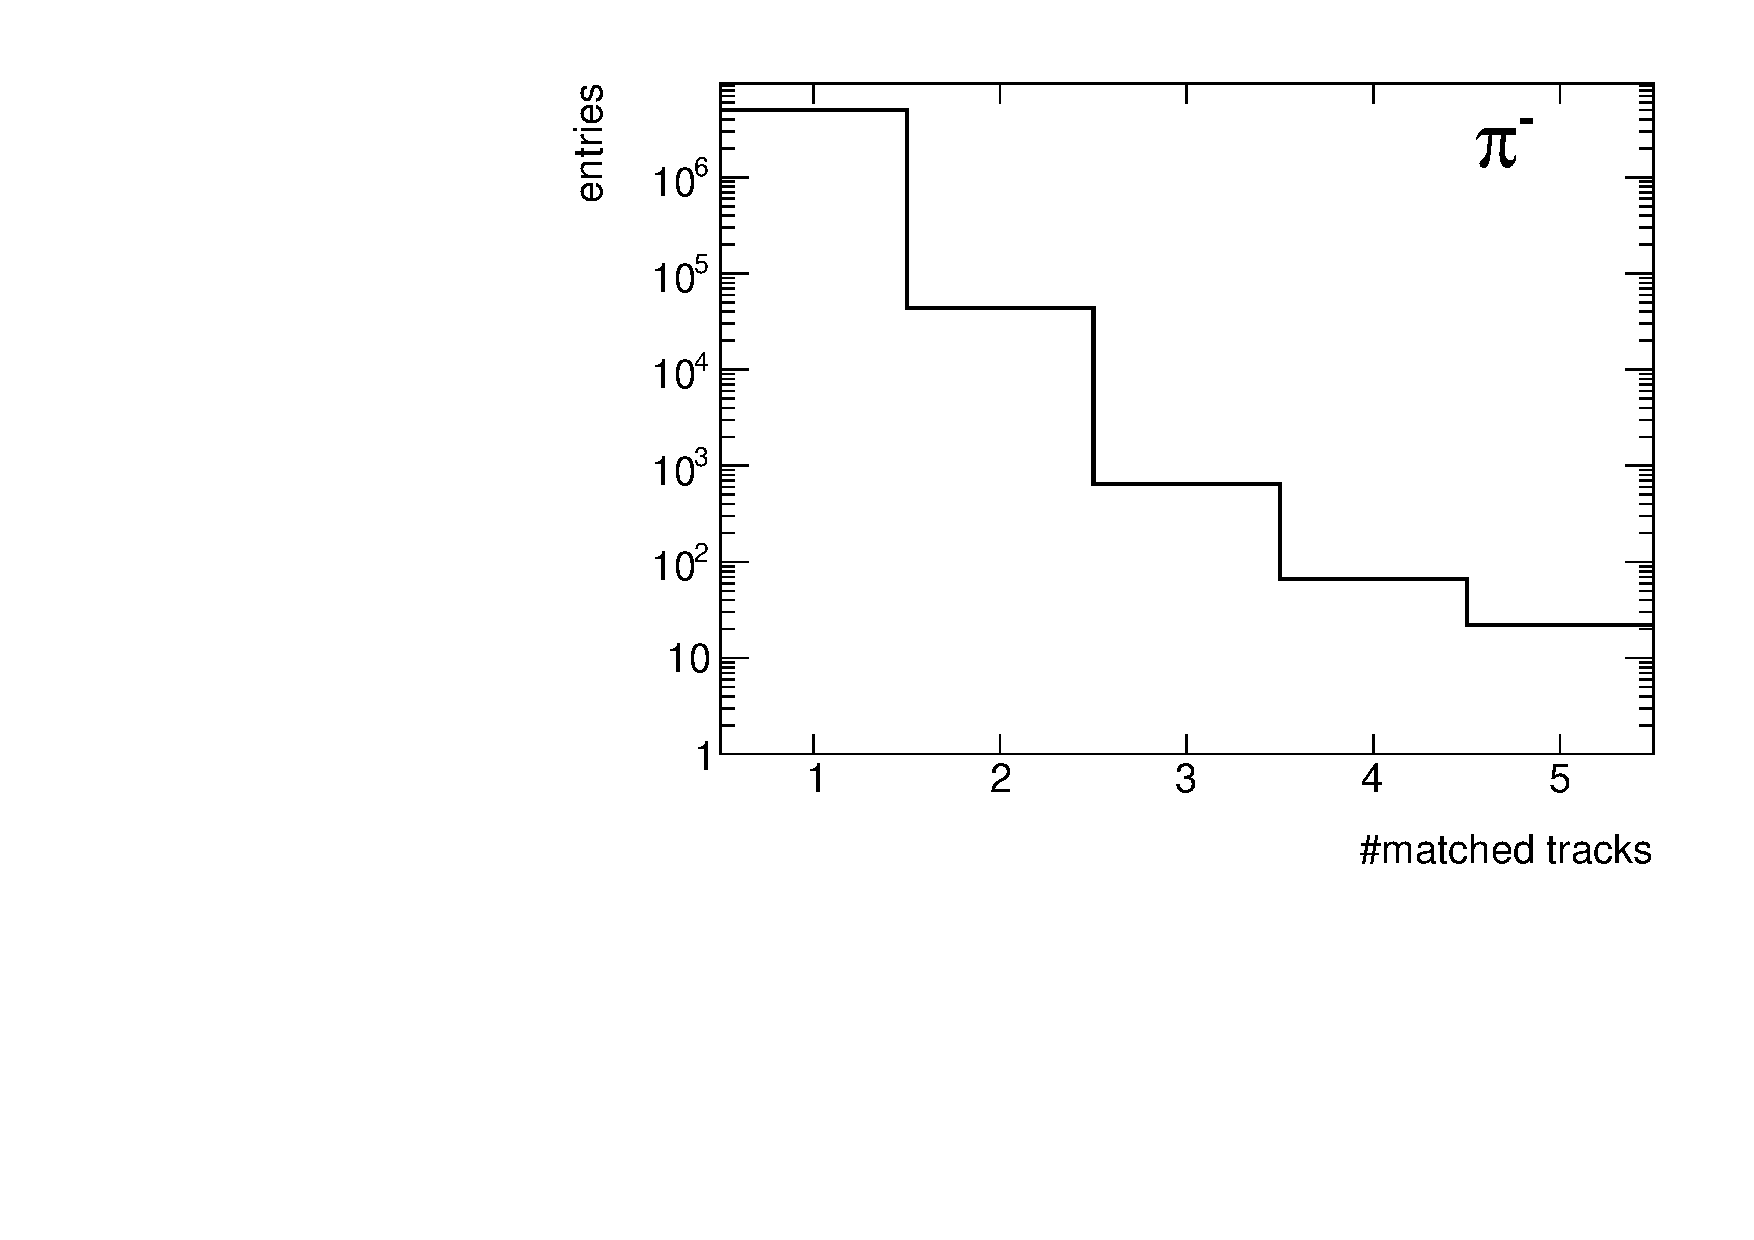
\includegraphics[width=\linewidth,page=1]{graphics/eff/trackSplitting_CD.pdf}\\
		\includegraphics[width=\linewidth,page=4]{graphics/eff/trackSplitting_CD.pdf}\\
	}~
	\parbox{0.329\textwidth}{
		\centering
		\includegraphics[width=\linewidth,page=2]{graphics/eff/trackSplitting_CD.pdf}\\
		\includegraphics[width=\linewidth,page=5]{graphics/eff/trackSplitting_CD.pdf}\\
	}%
	\parbox{0.329\textwidth}{
		\centering
		\includegraphics[width=\linewidth,page=3]{graphics/eff/trackSplitting_CD.pdf}\\
		\includegraphics[width=\linewidth,page=6]{graphics/eff/trackSplitting_CD.pdf}\\
	}%
	\caption[Number of reconstructed global tracks, satisfying all quality criteria, matched with the same true level primary particle.]{Number of reconstructed global tracks, satisfying all quality criteria (cuts~\ref{sec:TpcQualityCuts}), matched with the~same true level primary particle. The type of true level particle is indicated in the figure.}\label{fig:trackSplittingNominal}
\end{figure}

The true level particle end vertex $V_r^{end}$ is not specified if the particle neither interacted with the dead material nor decayed. The analysis showed that $1\%$ of the reconstructed tracks are matched to the true particle which lost identitiy ($V_r^{end}<48$~cm) before entering TPC. We interprate such situation as matching of reconstructed daugther particle to true level parent particle. It is potentially dangerous since  momentum and type of daugther particle might be different from parent particle.  Problem with wrong true level matching is also present for tracks with only one track matched to true level particle which do not decay or interact with material (no end vertex assosiated to true  level particle). 
It is visible on Fig.~\ref{fig:trackSplittingNominaldEdx} where $dE/dx$ is shown that some reconstracted tracks 
have different PID than true level particle matched to it.
 Also, there are problems in the closure tests, where  the  reconstructed-level distributions of rapidity and transverse momenta weighted by the nominal efficiency corrections do not describe the true level distributions. Main reason for failing of closure tests is non-negligible (and significant   for anti-protons) amount of global tracks matched with primary particles but no or little correlation in $\eta-\phi$ space beetwen
matched pair. 
The~distance 
\begin{equation}\label{eq:tpcMatchingDeltaSquare}
\delta^{2}\left(\eta,\phi\right)=\left(\eta^{true}-\eta^{reco}\right)^2+\left(\phi^{true}-\phi^{reco}\right)^2
\end{equation}
between the true level particle and global track assigned to it, shown in Fig.~\ref{fig:trackSplittingNominalDelta_1} for particles with only one  matched global track and Fig.~\ref{fig:trackSplittingNominalDelta_2} for particles with at least two  matched global tracks, indicates that some part of the tracks taken for the efficiency calculation are measured very badly ($\delta^{2}\left(\eta,\phi\right)$ is very large), even if there is only one global track matched to the true-particle.
\begin{figure}[ht]
	\centering
	\parbox{0.329\textwidth}{
		\centering
		\includegraphics[width=\linewidth,page=31]{graphics/eff/trackSplitting_CD.pdf}\\
		\includegraphics[width=\linewidth,page=34]{graphics/eff/trackSplitting_CD.pdf}\\
	}~
	\parbox{0.329\textwidth}{
		\centering
		\includegraphics[width=\linewidth,page=32]{graphics/eff/trackSplitting_CD.pdf}\\
		\includegraphics[width=\linewidth,page=35]{graphics/eff/trackSplitting_CD.pdf}\\
	}%
	\parbox{0.329\textwidth}{
		\centering
		\includegraphics[width=\linewidth,page=33]{graphics/eff/trackSplitting_CD.pdf}\\
		\includegraphics[width=\linewidth,page=36]{graphics/eff/trackSplitting_CD.pdf}\\
	}%
	\caption[$dE/dx$ of the track matched to true level particle.]{$dE/dx$ of the track matched to true level particle. Lines indicate Bichsel function prediction for each particle species. Only tracks matched to non-interacting true level particles without end vertex  are shown.}\label{fig:trackSplittingNominaldEdx}
\end{figure}

Because of several above mentioned  problems with  nominal STAR definition of matching between reconstructed tracks and true  level particles we decided to use in the analysis modified matching            
definition by taking into the account the difference    between reconstructed tracks and true particles in $\eta-\phi$ space.




\begin{figure}[hb]
	\centering
	\parbox{0.329\textwidth}{
		\centering
		\includegraphics[width=\linewidth,page=25]{graphics/eff/trackSplitting_CD.pdf}\\
		\includegraphics[width=\linewidth,page=28]{graphics/eff/trackSplitting_CD.pdf}\\
	}~
	\parbox{0.329\textwidth}{
		\centering
		\includegraphics[width=\linewidth,page=26]{graphics/eff/trackSplitting_CD.pdf}\\
		\includegraphics[width=\linewidth,page=29]{graphics/eff/trackSplitting_CD.pdf}\\
	}%
	\parbox{0.329\textwidth}{
		\centering
		\includegraphics[width=\linewidth,page=27]{graphics/eff/trackSplitting_CD.pdf}\\
		\includegraphics[width=\linewidth,page=30]{graphics/eff/trackSplitting_CD.pdf}\\
	}%
	\caption[$\delta^{2}\left(\eta,\phi\right)$ distributions between true level particles and tracks assigned to them.]{$\delta^{2}\left(\eta,\phi\right)$ distributions  between true level particles and tracks assigned to them. Only true level particles with only one reconstructed track matched to them were selected. Red lines and arrows indicate  the~cut value of $0.15^2$, which is used in the modified true level particle-track matching definition.}\label{fig:trackSplittingNominalDelta_1}
\end{figure}

\begin{figure}[h!]\vspace{-10pt}
	\centering
	\parbox{0.329\textwidth}{
		\centering
		\includegraphics[width=\linewidth,page=19]{graphics/eff/trackSplitting_CD.pdf}\\
		\includegraphics[width=\linewidth,page=22]{graphics/eff/trackSplitting_CD.pdf}\\
	}~
	\parbox{0.329\textwidth}{
		\centering
		\includegraphics[width=\linewidth,page=20]{graphics/eff/trackSplitting_CD.pdf}\\
		\includegraphics[width=\linewidth,page=23]{graphics/eff/trackSplitting_CD.pdf}\\
	}%
	\parbox{0.329\textwidth}{
		\centering
		\includegraphics[width=\linewidth,page=21]{graphics/eff/trackSplitting_CD.pdf}\\
		\includegraphics[width=\linewidth,page=24]{graphics/eff/trackSplitting_CD.pdf}\\
	}%
	\caption[$\delta^{2}\left(\eta,\phi\right)$ distributions between true level particles and tracks assigned to them.]{$\delta^{2}\left(\eta,\phi\right)$ distributions between true level particles and tracks assigned to them. Only true level particles with at least two reconstructed tracks matched to them were selected. Red lines and arrows indicate  the~cut value of $0.15^2$, which is used in the modified true level particle-track matching definition.}\label{fig:trackSplittingNominalDelta_2}
\end{figure}




\subsection{Method used in this analysis}\label{subsec:definitionTrueLevelMatching}
In this method, the definition of true level particle-track matching is modified. In addition to the requirement of the appropriate number of common hit points, the distance between true level particle and track is required to be smaller than $0.15$, $\delta^{2}\left(\eta,\phi\right)<\left(0.15\right)^2$. It is quite an arbitrary value which should be small but not too small  to loose good events. The value of $\delta^2$ cut was chosen by the requirement that only acceptable small amount of CEP events which passed all selection criteria will not satisfy matching criteria. It was verified with the CEP MC embedded into zero-bias triggers that with quoted value of cut on $\delta^{2}\left(\eta,\phi\right)$ less than $0.3\%$ of CEP events have at least one track which is not considered to be matched with true-level pion despite the standard matching (Fig.~\ref{fig:deltaSqCEP}). We consider this an acceptably low effect.

Tracks, which do not satisfy the above criterion, are treated as fake tracks (even if they are matched to the true level particle in the standard way). In almost all cases, where the $\delta^{2}\left(\eta,\phi\right)<\left(0.15\right)^2$, there is only one track matched to true level particle (Fig.~\ref{fig:trackSplittingetaPhi}). Additionally, the $dE/dx$ of the track is mostly consistent with the true level PID (Fig.~\ref{fig:trackSplittingEtaPhidEdx}). Figure~\ref{fig:trackTPCefficiencyComparisonEtaPhi} shows the difference between TPC efficiencies obtained with the STAR standard and the modified definition of true particle-track matching.


%---------------------------
\begin{figure}[h!]%\vspace{-10pt}
	\centering
	\parbox{0.685\textwidth}{
		\centering
		\begin{subfigure}[b]{\linewidth}
			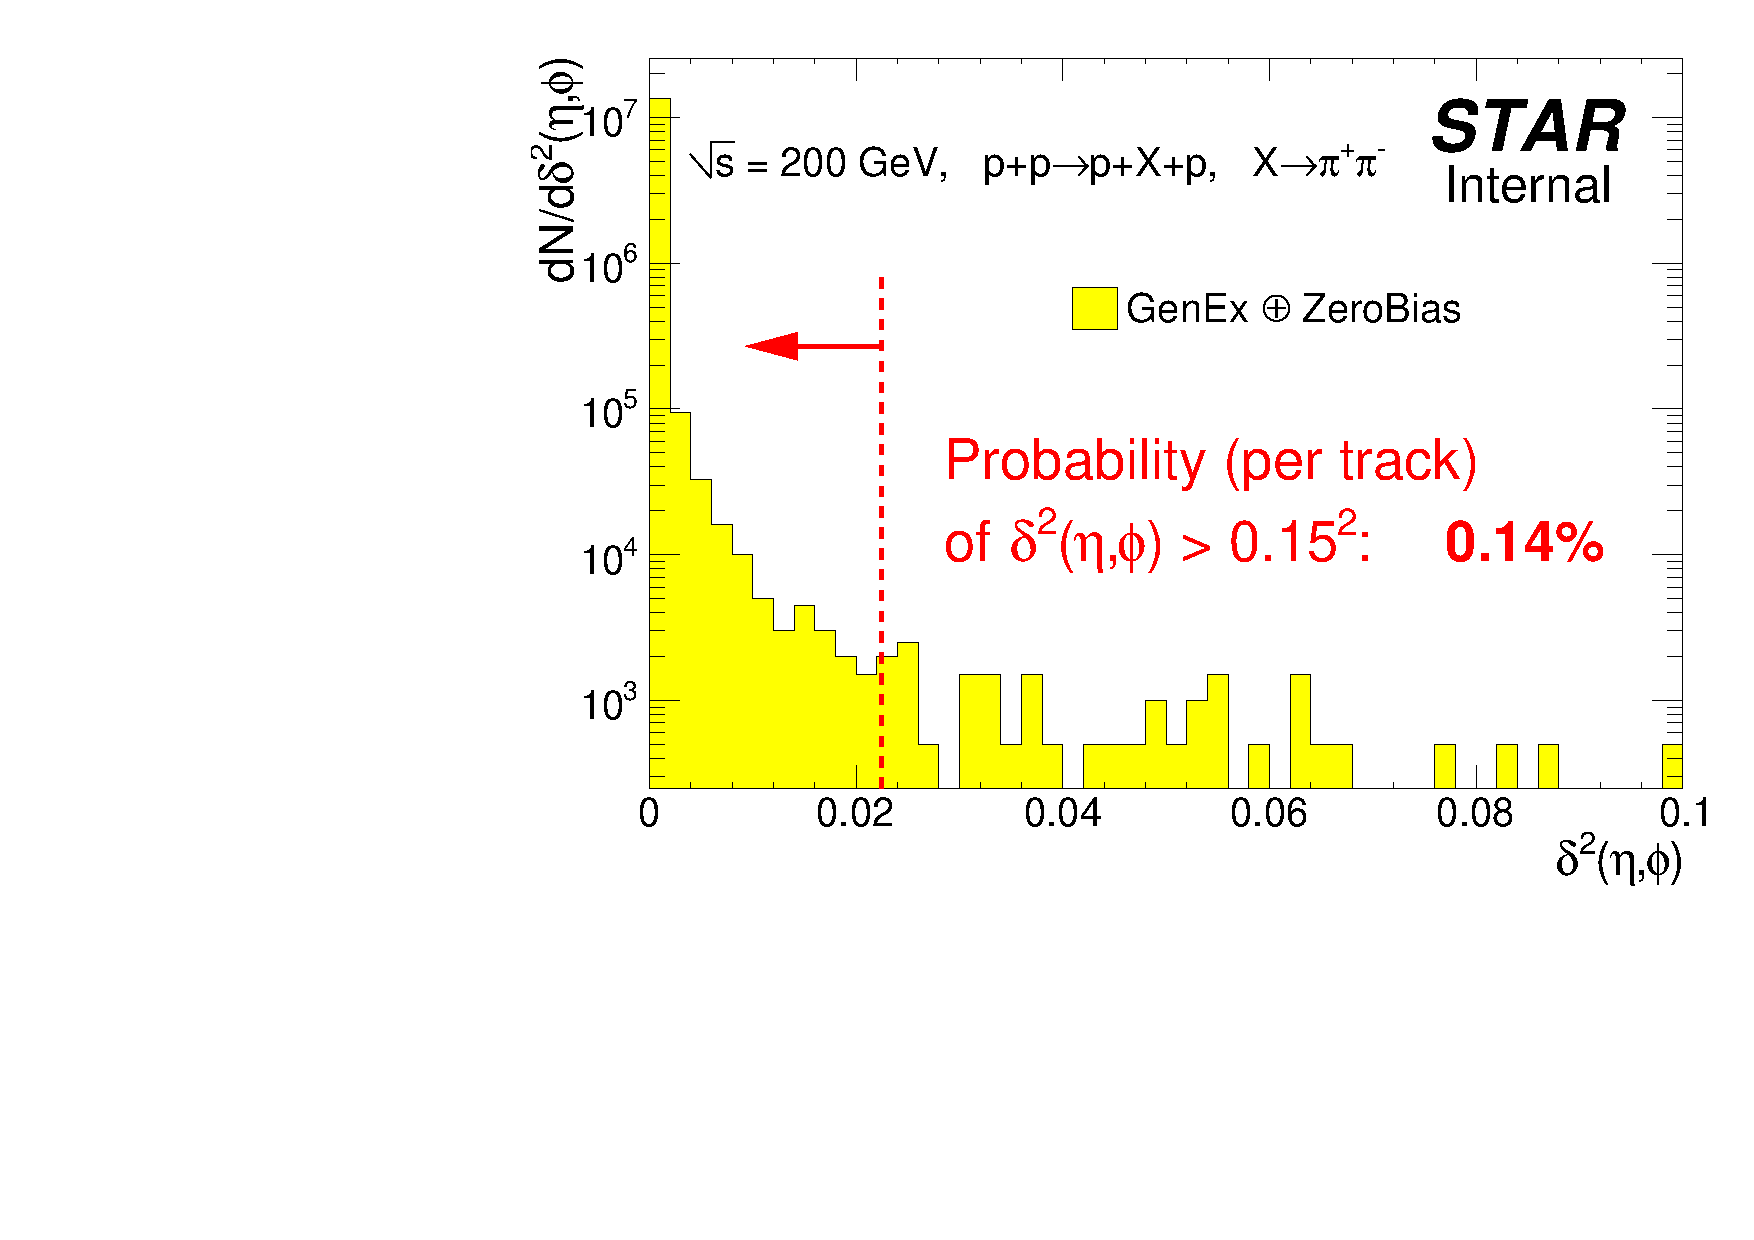
\includegraphics[width=\linewidth]{graphics/eff/deltaEtaSqDeltaPhiSqMatchedExclusive.pdf}
		\end{subfigure}
	}%
	\quad%
	\parbox{0.285\textwidth}{
		\centering
		\begin{minipage}[t][0.78\linewidth][t]{\linewidth}\vspace{-60pt}
			\caption[Distribution of $\delta^{2}\left(\eta,\phi\right)$ in CEP MC.]%
			{Distribution of $\delta^{2}\left(\eta,\phi\right)$ for tracks matched with true-level pions (using standard matching) in CEP MC embedded into zero-bias triggers. Tracks were taken from events passing full CEP event selection, recognized as exclusive $\pi^{+}\pi^{-}$. The vertical red dashed line indicates the cut value of $0.15^{2} \approx 0.023$, above which less than 0.14\% of tracks is contained.}%
			\label{fig:deltaSqCEP}
		\end{minipage}
	}
\end{figure}
%---------------------------


\begin{figure}[ht]
	\centering
	\parbox{0.329\textwidth}{
		\centering
		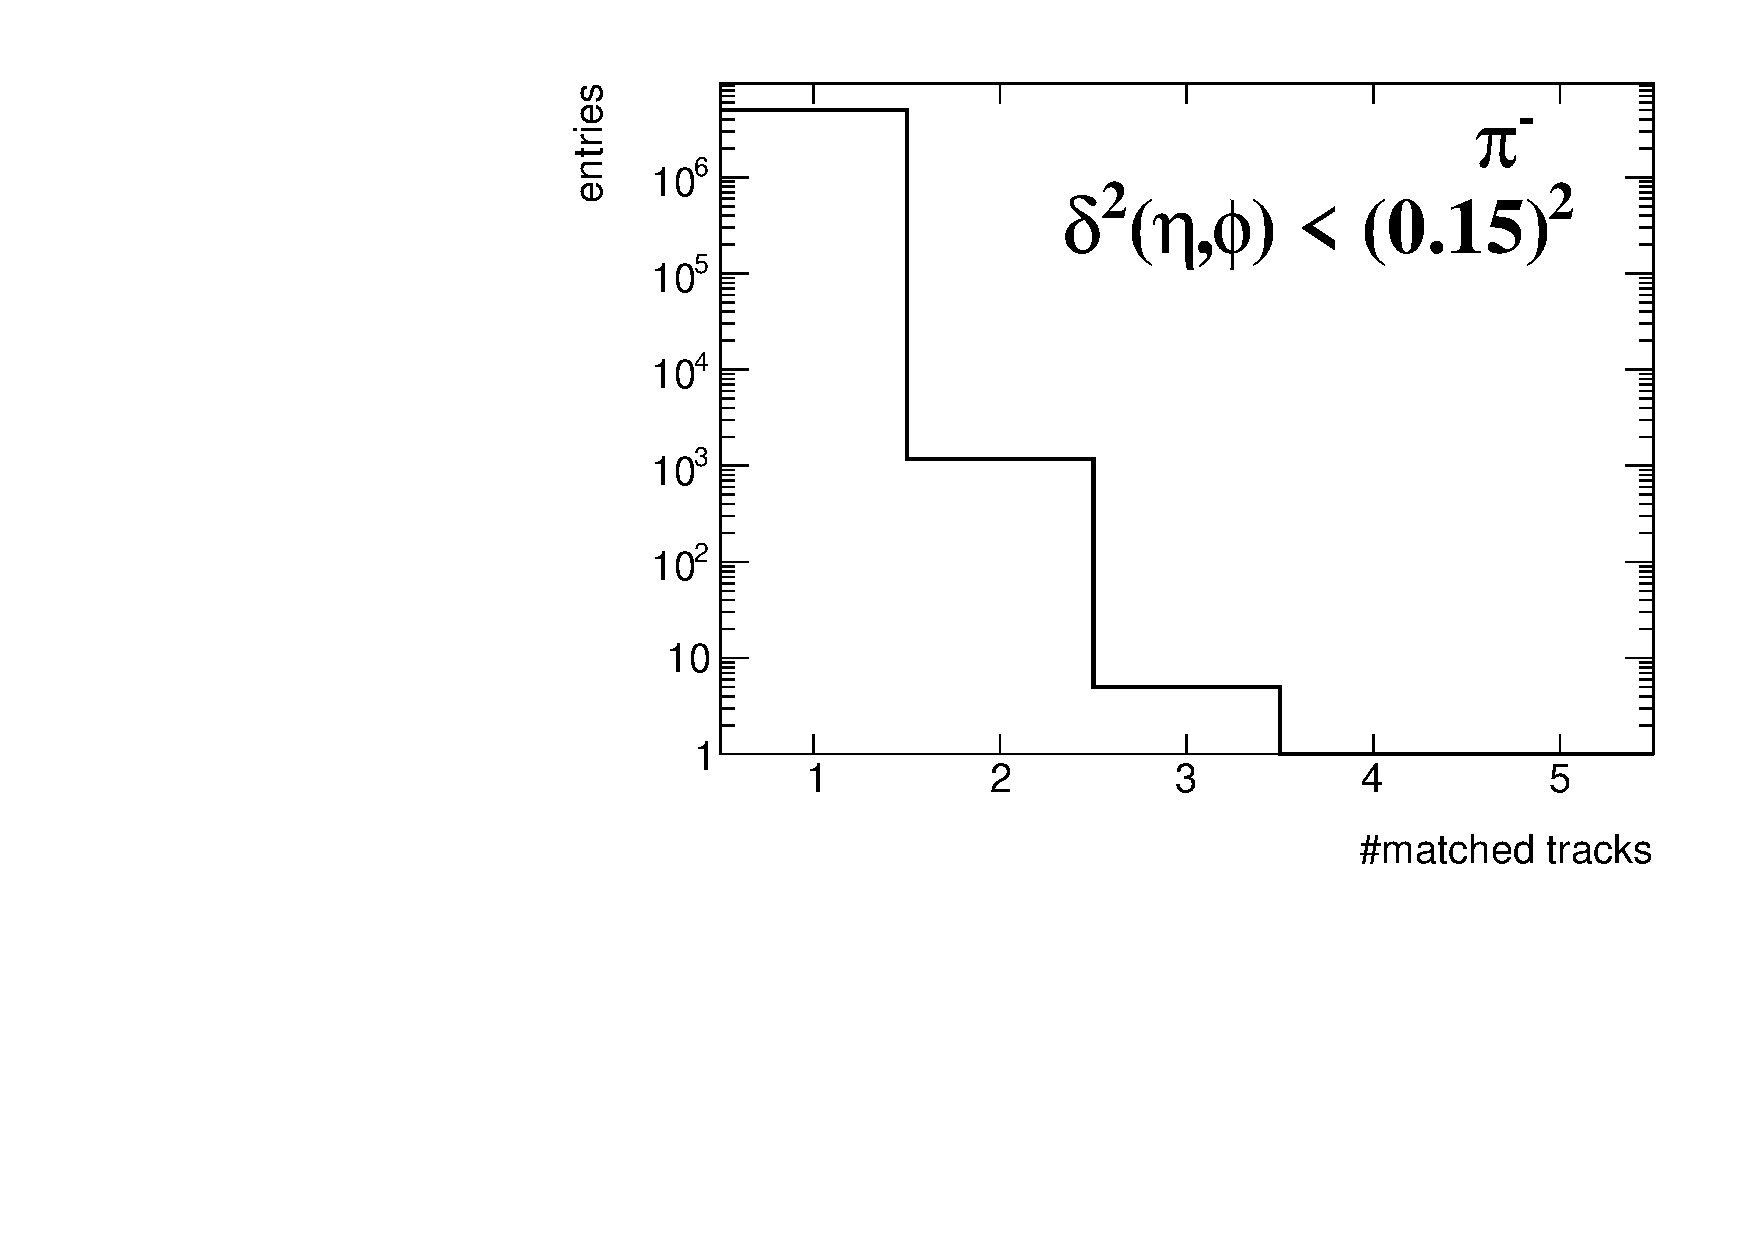
\includegraphics[width=\linewidth,page=1]{graphics/eff/trackSplitting_QualityEtaPhiCD.pdf}\\
		\includegraphics[width=\linewidth,page=4]{graphics/eff/trackSplitting_QualityEtaPhiCD.pdf}\\
	}~
	\parbox{0.329\textwidth}{
		\centering
		\includegraphics[width=\linewidth,page=2]{graphics/eff/trackSplitting_QualityEtaPhiCD.pdf}\\
		\includegraphics[width=\linewidth,page=5]{graphics/eff/trackSplitting_QualityEtaPhiCD.pdf}\\
	}%
	\parbox{0.329\textwidth}{
		\centering
		\includegraphics[width=\linewidth,page=3]{graphics/eff/trackSplitting_QualityEtaPhiCD.pdf}\\
		\includegraphics[width=\linewidth,page=6]{graphics/eff/trackSplitting_QualityEtaPhiCD.pdf}\\
	}%
	\caption[Number of reconstructed global tracks, satisfying all quality criteria and $\delta^{2}\left(\eta,\phi\right)$ cut, matched with the same true level primary particle.]{Number of reconstructed global tracks, satisfying all quality criteria (cuts~\ref{sec:TpcQualityCuts}) and $\delta^{2}\left(\eta,\phi\right)$ cut, matched with the same true level primary particle.}\label{fig:trackSplittingetaPhi}
\end{figure}


\begin{figure}[h!]%\vspace{-5pt}
	\centering
	\parbox{0.329\textwidth}{
		\centering
		\includegraphics[width=\linewidth,page=21]{graphics/eff/trackSplitting_QualityEtaPhiCD.pdf}\\
		\includegraphics[width=\linewidth,page=24]{graphics/eff/trackSplitting_QualityEtaPhiCD.pdf}\\
	}~
	\parbox{0.329\textwidth}{
		\centering
		\includegraphics[width=\linewidth,page=22]{graphics/eff/trackSplitting_QualityEtaPhiCD.pdf}\\
		\includegraphics[width=\linewidth,page=25]{graphics/eff/trackSplitting_QualityEtaPhiCD.pdf}\\
	}%
	\parbox{0.329\textwidth}{
		\centering
		\includegraphics[width=\linewidth,page=23]{graphics/eff/trackSplitting_QualityEtaPhiCD.pdf}\\
		\includegraphics[width=\linewidth,page=26]{graphics/eff/trackSplitting_QualityEtaPhiCD.pdf}\\
	}%
	\caption[$dE/dx$ of the closest track matched to true level particle passing the $\delta^{2}\left(\eta,\phi\right)$ cut.]{$dE/dx$ of the closest track matched to true level particle passing the $\delta^{2}\left(\eta,\phi\right)$ cut. Lines indicate Bichsel function prediction for each particle species.}\label{fig:trackSplittingEtaPhidEdx}
\end{figure}

\begin{figure}[ht]%[hb]
	\centering
	\parbox{0.329\textwidth}{
		\centering
		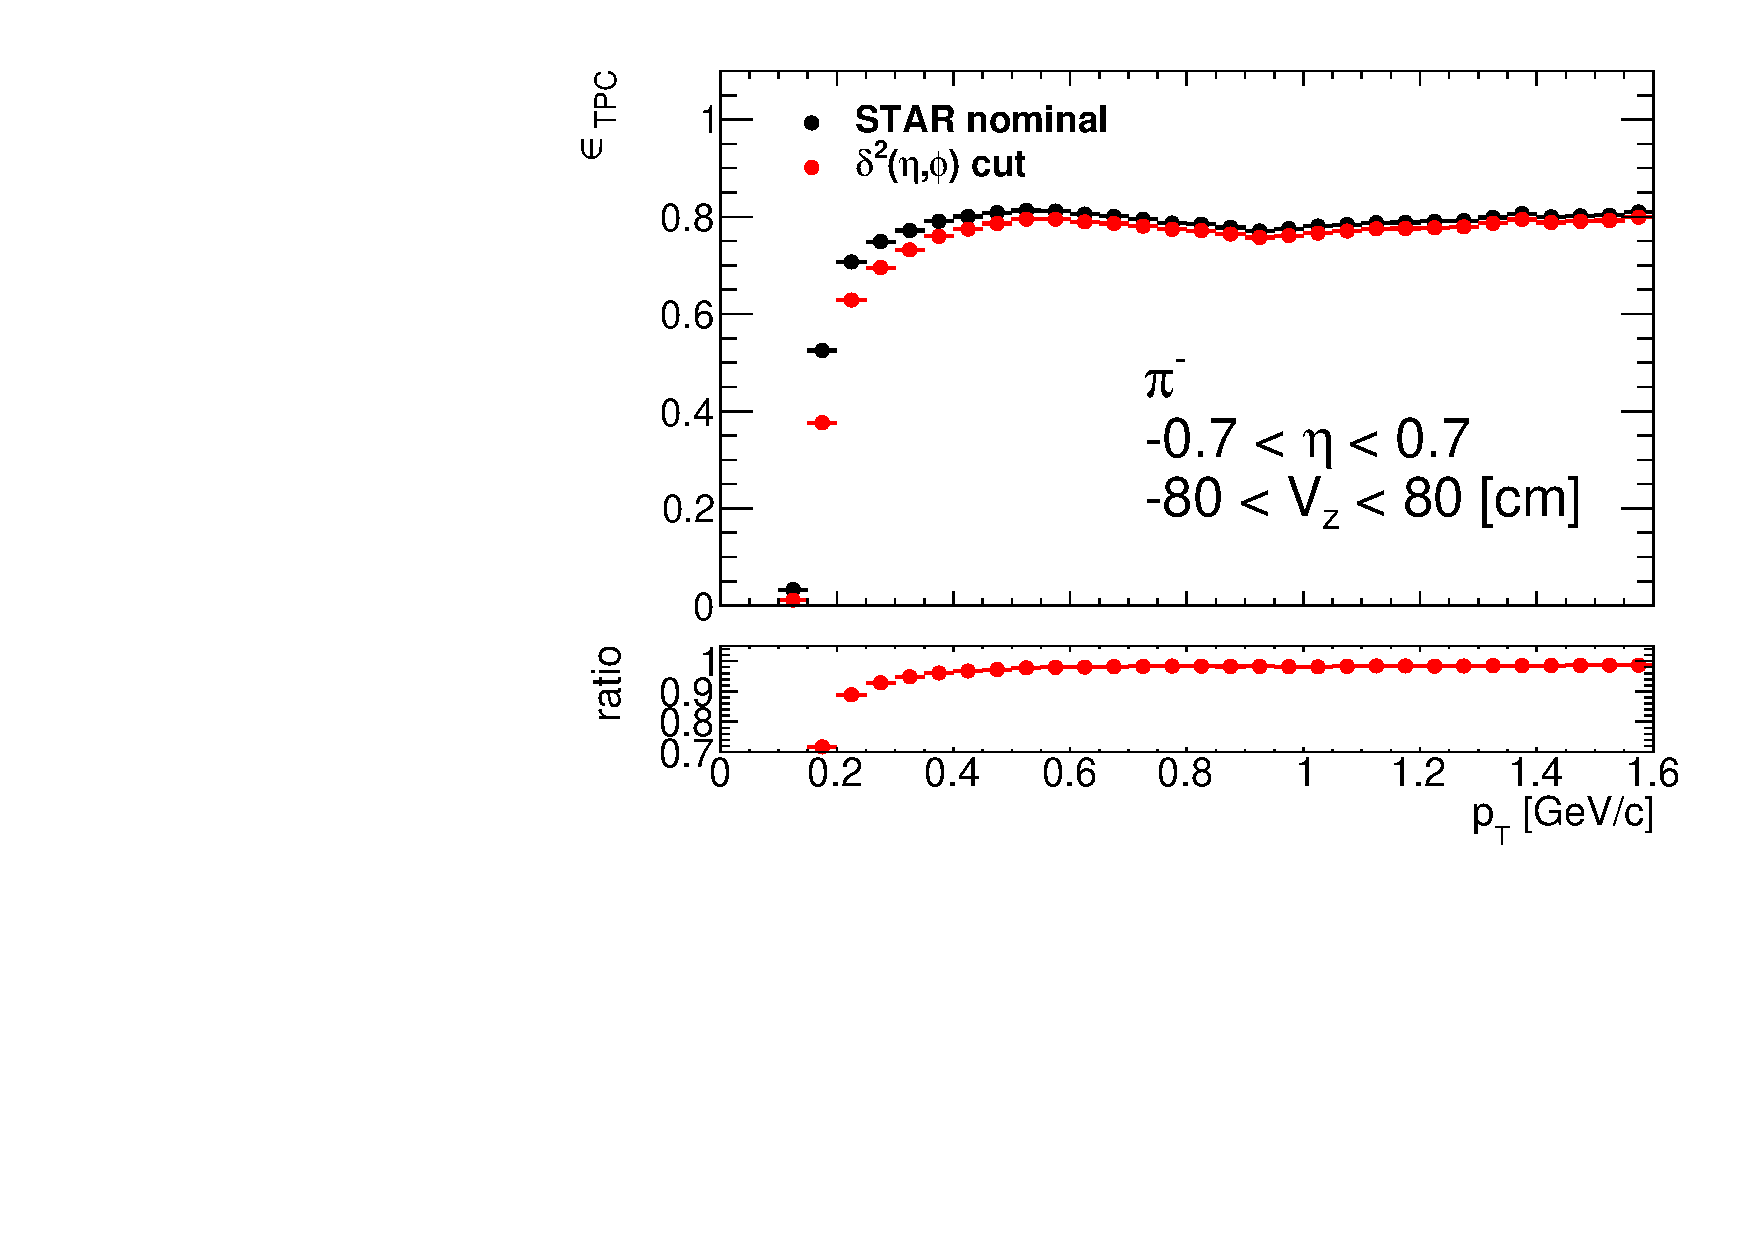
\includegraphics[width=\linewidth,page=1]{graphics/eff/tpcEffi.pdf}\\
		\includegraphics[width=\linewidth,page=4]{graphics/eff/tpcEffi.pdf}\\
	}~
	\parbox{0.329\textwidth}{
		\centering
		\includegraphics[width=\linewidth,page=2]{graphics/eff/tpcEffi.pdf}\\
		\includegraphics[width=\linewidth,page=5]{graphics/eff/tpcEffi.pdf}\\
	}%
	\parbox{0.329\textwidth}{
		\centering
		\includegraphics[width=\linewidth,page=3]{graphics/eff/tpcEffi.pdf}\\
		\includegraphics[width=\linewidth,page=6]{graphics/eff/tpcEffi.pdf}\\
	}%
	\caption[TPC acceptance and reconstruction efficiency as a function of $p_T$ $\left(|V_z|<80\textrm{ cm}, |\eta|<0.7\right)$ obtained from two methods.]{TPC acceptance and reconstruction efficiency as a function of $p_T$ $\left(|V_z|<80\textrm{ cm}, |\eta|<0.7\right)$ obtained from two methods.}\label{fig:trackTPCefficiencyComparisonEtaPhi}
\end{figure}


\subsection{Sample of  efficiency plots}\label{subsec:sampleTpcEffPlots}

In Figure~\ref{fig:tpcEff_pion_sample} we present sample plots of the TPC track and reconstruction efficiency calculated with modified definition of reconstructed track and true-level particle matching (according to description in Sec.~\ref{subsec:definitionTrueLevelMatching}), used in our analyses. Plots for all analyzed particle types and all bins of true $z_{\text{vtx}}$ are contained in Appendix~\ref{appendix:tpcEff}.

In order to maximize the statistics available for the measurement (possibly wide range of accepted longitudinal vertex position $z_{\text{vtx}}$) with maximized probed phase-space in analyzed physics processes (wide range of track $p_{T}$ and $\eta$) and minimized systematic uncertainties related to the central detector (TPC and TOF), we have studied the efficiency plots like ones shown in Fig.~\ref{fig:tpcEff_pion_sample} and Fig.~\ref{fig:tofEff_pion_sample}. We thus decided to set the cut on $z_{\text{vtx}}$ at $\pm80~\text{cm}$, which corresponds to 89\% of the full integral of normal distribution with mean at 0 and standard deviation of 50~cm. At the same time we set the cuts on track $p_{T}$ and $\eta$ as listed in Sec.~\ref{sec:TpcKinematicCuts}. These cuts are represented with red dashed lines in Fig.~\ref{fig:tpcEff_pion_sample} and Fig.~\ref{fig:tofEff_pion_sample}. Our goal was to operate within cuboid ($z_{\text{vtx}}$, $p_{T}$, $\eta$) region of relatively high TPC and TOF efficiency ($\geq50\%$ of the maximum value). In other words, we required high acceptance and efficiency for a rectangular ($p_{T}$, $\eta$) space with limits independent from $z_{\text{vtx}}$. One can see that the red lines in Fig.~\ref{fig:tpcEff_pion_sample} and Fig.~\ref{fig:tofEff_pion_sample} always contain in their interior the region of relatively high acceptance.

%---------------------------
\begin{figure}[h!]%\vspace{-10pt}
	\centering
	\parbox{0.485\textwidth}{
		\centering
		\begin{subfigure}[b]{\linewidth}
			\subcaptionbox{\label{fig:tpcEff_pion_sample_a}}{\includegraphics[width=\linewidth,page=3]{graphics/eff/Eff2D_TPC_pion_Minus.pdf}\vspace*{-8pt}}
		\end{subfigure}\\[5pt]
		\begin{subfigure}[b]{\linewidth}\addtocounter{subfigure}{1}
			\subcaptionbox{\label{fig:tpcEff_pion_sample_c}}{\includegraphics[width=\linewidth,page=18]{graphics/eff/Eff2D_TPC_pion_Minus.pdf}\vspace*{-8pt}}
		\end{subfigure}
	}%
	\quad%
	\parbox{0.485\textwidth}{
		\centering
		\begin{subfigure}[b]{\linewidth}\addtocounter{subfigure}{-2}
			\subcaptionbox{\label{fig:tpcEff_pion_sample_b}}{\includegraphics[width=\linewidth,page=11]{graphics/eff/Eff2D_TPC_pion_Minus.pdf}\vspace*{-8pt}}
		\end{subfigure}\\[5pt]
		\begin{minipage}[t][0.78\linewidth][t]{\linewidth}\vspace{10pt}
		\caption[Sample TPC acceptance and reconstruction efficiency of $\pi^{-}$.]{Sample TPC acceptance and reconstruction efficiency of $\pi^{-}$ in 3 bins of true $z_{\text{vtx}}$. Plots represent the TPC efficiency $\epsilon_{\text{TPC}}$ ($z$-axis) as a function of true particle pseudorapidity $\eta$ ($x$-axis) and transverse momentum $p_{T}$ ($y$-axis) in single $z$-vertex bin whose range is given at the top. Red lines and arrows indicate region accepted in analyses.}\label{fig:tpcEff_pion_sample}
		\end{minipage}
	}
\end{figure}
%---------------------------





\section{TOF acceptance, hit reconstruction and track matching efficiency}\label{sec:tofMatchEff}

Combined TOF acceptance, hit reconstruction efficiency and matching efficiency with TPC tracks, $\epsilon_{\textrm{\tiny TOF}}$, was defined as the probability that the global TPC track that satisfy quality criteria (cuts~\ref{sec:TpcQualityCuts}) is matched with hit in TOF (\ref{sec:TpcTofMatchingRequirement}). This quantity is generally referred as ``TOF efficiency''.

It was calculated in the very similiar way to TPC efficiency - single particle STARsim MC embedded into zero-bias triggers was used. Tracks belonging to $set~B$ from Sec.~\ref{sec:tpcAccAndEff} were utilized. From these tracks a sub-sample of tracks with non-zero TOF matching flag (StMuBTofPidTraits.mMatchFlag $>0$) was extracted ($set~C$). The TOF efficiency was calculated as
\begin{equation}\label{eq:tofAccAndEffDefinition}
		\epsilon_{\textrm{\tiny TOF}}\left(p_{T}, \eta, z_{vtx};~\textrm{sign},\textrm{PID}\right) = \frac{(p_{T},\eta, z_{vtx})~\textrm{histogram for particles of given sign and ID from}~set~C}{(p_{T},\eta, z_{vtx})~\textrm{histogram for particles of given sign and ID from}~set~B}.
	\end{equation}

An additional note has to be made here about the correction which is applied to TOF matching flag in MC analysis. It was found that in embedded simulation the dead TOF elements were not masked. To correct for this effect (hence obtain more reliable TOF efficiency) a data-based map of modules was created, separately for each RHIC fill. Map was filled with modules which were matched with TPC tracks in the data. In all MC sample analyses (including efficiency determination) each TPC track with non-zero TOF match flag was additionally checked if TOF module that track was matched with had any entries in the data-based map. If not - the TOF match flag was considered 0.

\subsection{Sample of  efficiency plots}

The sample TOF efficiency plot is shown in Fig.~\ref{fig:tofEff_pion_sample}. All remaining TOF efficiency plots are contained in Appendix~\ref{appendix:tofEff}.

As shown in Sec.~\ref{sec:tofAbsEffCorr} the data-driven efficiency and MC effficiency differ significantly, therefore the final TOF efficiency which is used to correct the data is the presented here (taken from single particle embedded MC) but additionally modified according to correction derived in the reffered section.

%---------------------------
\begin{figure}[H]%\vspace{-10pt}
	\centering
	\parbox{0.485\textwidth}{
		\centering
		\begin{subfigure}[b]{\linewidth}
			\subcaptionbox{\label{fig:tofEff_pion_sample_a}}{\includegraphics[width=\linewidth,page=3]{graphics/eff/Eff2D_TOF_pion_Minus.pdf}\vspace*{-8pt}}
		\end{subfigure}\\[5pt]
		\begin{subfigure}[b]{\linewidth}\addtocounter{subfigure}{1}
			\subcaptionbox{\label{fig:tofEff_pion_sample_c}}{\includegraphics[width=\linewidth,page=18]{graphics/eff/Eff2D_TOF_pion_Minus.pdf}\vspace*{-8pt}}
		\end{subfigure}
	}%
	\quad%
	\parbox{0.485\textwidth}{
		\centering
		\begin{subfigure}[b]{\linewidth}\addtocounter{subfigure}{-2}
			\subcaptionbox{\label{fig:tofEff_pion_sample_b}}{\includegraphics[width=\linewidth,page=11]{graphics/eff/Eff2D_TOF_pion_Minus.pdf}\vspace*{-8pt}}
		\end{subfigure}\\[5pt]
		\begin{minipage}[t][0.78\linewidth][t]{\linewidth}\vspace{10pt}
			\caption[Sample plotz of TOF acceptance, reconstruction and matching efficiency of $\pi^{-}$.]{Sample TOF acceptance, reconstruction and matching efficiency of $\pi^{-}$ in 3 bins of true $z_{\text{vtx}}$. Plots represent the TOF efficiency $\epsilon_{\text{TOF}}$ ($z$-axis) as a function of true particle pseudorapidity $\eta$ ($x$-axis) and transverse momentum $p_{T}$ ($y$-axis) in single $z$-vertex bin whose range is given at the top. Red lines and arrows indicate region accepted in analyses.}\label{fig:tofEff_pion_sample}
		\end{minipage}
	}
\end{figure}
%---------------------------

%---------------------------
%\begin{figure}[hb]%
%\centering\includegraphics[width=0.7\linewidth,page=11]{graphics/eff/Eff2D_TOF_pion_Minus.pdf}%
%\caption[Sample plot of TOF acceptance, reconstruction and matching efficiency of $\pi^{-}$.]{Sample plot of TOF acceptance, reconstruction and matching efficiency of $\pi^{-}$. Plot represents the TOF efficiency $\epsilon_{\text{TOF}}$ ($z$-axis) as a function of true particle pseudorapidity $\eta$ ($x$-axis) and transverse momentum $p_{T}$ ($y$-axis) in single $z$-vertex bin whose range is given at the top. Red lines and arrows indicate region accepted in analyses.}\label{fig:tofEff_pion_sample}
%\end{figure}
%---------------------------


% 
% \section{TPC vertex reconstruction efficiency}\label{sec:tpcVxRecoEff}
% 
% The definition of vertex reconstruction efficiency established in this analysis is the probability that two global tracks, both associated with true level primary particles from the kinematic region of the measurement, both satisfying kinematic and quality criteria (cuts~\ref{sec:TpcKinematicCuts} and ~\ref{sec:TpcQualityCuts}) and both matched with hits in TOF, form a vertex listed in the collection of reconstructed primary vertices and DCA(R) and DCA(z) of both global tracks calculated w.r.t. this vertex is contained within the limits of cut~\ref{sec:TpcDcaCuts}.


%% =====  ROMAN POT SIMULATION ====
%%===========================================================%%
%%                                                           %%
%%                  ROMAN POT SIMULATION                     %%
%%                                                           %%
%%===========================================================%%


\chapter{Roman Pot simulation}\label{chap:romanPotSimulation}


\begin{figure}[hb]%
\caption[Apertures.]{Apertures.}\label{fig:aperturesWithFit}%
\centering
\parbox{0.495\textwidth}{
  \centering
  \includegraphics[width=\linewidth,page=1]{graphics/rpSim/Apertures_swapedAxes_withFit_beforeDxShift.pdf}\\
  \includegraphics[width=\linewidth,page=2]{graphics/rpSim/Apertures_swapedAxes_withFit_beforeDxShift.pdf}\\
  \includegraphics[width=\linewidth,page=3]{graphics/rpSim/Apertures_swapedAxes_withFit_beforeDxShift.pdf}
}~
\parbox{0.495\textwidth}{
  \centering
  \includegraphics[width=\linewidth,page=1]{graphics/rpSim/Apertures_swapedAxes_withFit.pdf}\\
  \includegraphics[width=\linewidth,page=2]{graphics/rpSim/Apertures_swapedAxes_withFit.pdf}\\
  \includegraphics[width=\linewidth,page=3]{graphics/rpSim/Apertures_swapedAxes_withFit.pdf}
}%
\end{figure}
\begin{figure}[ht!]\ContinuedFloat
% ~\\[32pt]
\centering
\parbox{0.495\textwidth}{
  \centering
  \includegraphics[width=\linewidth,page=4]{graphics/rpSim/Apertures_swapedAxes_withFit_beforeDxShift.pdf}
}~
\parbox{0.495\textwidth}{
  \centering
  \includegraphics[width=\linewidth,page=4]{graphics/rpSim/Apertures_swapedAxes_withFit.pdf}
}%
\end{figure}
%---------------------------

%% =====  DE/DX CORRECTION ====
%%===========================================================%%
%%                                                           %%
%%                     DE/DX CORRECTION                      %%
%%                                                           %%
%%===========================================================%%


\chapter{\texorpdfstring{d$\bm{E}$/d$\bm{x}$}{dE/dx} correction}\label{chap:dEdxCorrection}

Particle identification in our analyses is done using merged information from the TPC (specific energy loss of tracks $dE/dx$) and from the TOF (time of hit macthed to TPC track). As can be seen in Fig.~\ref{fig:dEdxDataVsMC}, $dE/dx$ information from the MC events simulated in STARsim (in red) poorely matches the data points (black). This results e.g. in large systematic error of estimate of particle identification efficiency.

This problem was discussed under ticket \#3272~(Ref.~\cite{dedxTicket}). There were trials to improve the TPC calibration in simulation, but the problem remained. It was finally concluded that the origin of the problem lies in the model of energy loss used in the STARsim, therefore any further action was postponed. 

In order to tune simulated reposponse of the TPC in terms of $dE/dx$, hence also reduce the systematic uncertainty related to particle identification, a correction method was developed based on proper transformation (recalculation) of simulated $dE/dx$ to obtain new $dE/dx$ whose distribution matches the data.

It is possible to transform dE/dx in MC to make it follow the shape of dE/dx in the data. 
We know that $n^{\sigma}_{X}$ (where $X=\pi, K, p$, ...) variable follows a gaussian distribution (for particle X)
 \[n^{\sigma}_{X} = \Big( \ln{\frac{dE/dx}{\langle dE/dx\rangle_{X}}} \Big) / \sigma_{dE/dx},~~~~~f(n^{\sigma}_{X}) = \mathcal{N}(n^{\sigma}_{X}; \mu=0,\sigma=1)\]
therefore $dE/dx$ itself follows log-normal distribution:
\[f(dE/dx) = \mathcal{L}og\mathcal{N}(dE/dx; \mu=\langle dE/dx\rangle,\sigma=\sigma_{dE/dx}) = \frac{1}{\sqrt{2\pi}\cdot \sigma\cdot dE/dx}e^{-\frac{\ln^{2}{\frac{dE/dx}{\langle dE/dx\rangle}}}{2\sigma^{2}}}\]
The transformation we want to apply should preserve the shape of $dE/dx$ (so that it is still described by $\mathcal{L}og\mathcal{N}$), however it should change $\mu$ and $\sigma$ so that these values are euqal to those seen in the data. The transformation that satisfies above postulate is
\[dE/dx' = c\cdot (dE/dx)^{a}\]
Parameters of the distribution $\mathcal{L}og\mathcal{N}(dE/dx')$ would be then
\[\mu' = c\cdot\mu^{a},~~~~\sigma' = a\cdot\sigma\]
From above we get formulae for parameters of the transformation:
\[a=\sigma'/\sigma,~~~~c = \frac{\mu'}{\mu^{a}}\]

AlternativeToCrystallBall~\cite{AlternativeToCrystallBall}~Eq.~\eqref{eq:expTail}

\begin{equation}\label{eq:expTail}
	f(dE/dx)=\left\{
                \begin{array}{ll}
                  \frac{A}{\sqrt{2\pi}\cdot \sigma\cdot dE/dx}\exp{\Bigg(-\frac{1}{2}\Big(\frac{\ln{\frac{dE/dx}{\langle dE/dx\rangle}}}{\sigma}\Big)^{2}\Bigg)} & \textrm{for}~\frac{\ln{\frac{dE/dx}{\langle dE/dx\rangle}}}{\sigma} \leq k \\
                  \frac{A}{\sqrt{2\pi}\cdot \sigma\cdot dE/dx}\exp{\Bigg(-k\cdot \frac{\ln{\frac{dE/dx}{\langle dE/dx\rangle}}}{\sigma} + \frac{1}{2}k^{2} - k^{-1}\left(\frac{\frac{\ln{\frac{dE/dx}{\langle dE/dx\rangle}}}{\sigma}}{k}-1\right)^{k} \Bigg)} & \textrm{for}~\frac{\ln{\frac{dE/dx}{\langle dE/dx\rangle}}}{\sigma} > k
                \end{array}
              \right.
\end{equation}



%---------------------------
\begin{figure}[hb]
\centering
\parbox{0.495\textwidth}{
  \centering
  \includegraphics[width=\linewidth,page=4]{graphics/dedx/dEdx_fitPerMomentumBin_3rdIteration.pdf}\\
  \includegraphics[width=\linewidth,page=14]{graphics/dedx/dEdx_fitPerMomentumBin_3rdIteration.pdf}\\
  \includegraphics[width=\linewidth,page=24]{graphics/dedx/dEdx_fitPerMomentumBin_3rdIteration.pdf}\\
  \includegraphics[width=\linewidth,page=34]{graphics/dedx/dEdx_fitPerMomentumBin_3rdIteration.pdf}
}~
\parbox{0.495\textwidth}{
  \centering
  \includegraphics[width=\linewidth,page=9]{graphics/dedx/dEdx_fitPerMomentumBin_3rdIteration.pdf}\\
  \includegraphics[width=\linewidth,page=19]{graphics/dedx/dEdx_fitPerMomentumBin_3rdIteration.pdf}\\
  \includegraphics[width=\linewidth,page=29]{graphics/dedx/dEdx_fitPerMomentumBin_3rdIteration.pdf}\\
  \includegraphics[width=\linewidth,page=39]{graphics/dedx/dEdx_fitPerMomentumBin_3rdIteration.pdf}
}%
\caption[Fits to dE/dx spectra from the data.]{Fits of sum of functions from Eq.~\eqref{eq:expTail} corresponding to different particle species to dE/dx spectra from the data in a few momentum bins.}\label{fig:dEdxFits}
\end{figure}
%---------------------------



%---------------------------
\begin{figure}[hb]
\centering
\parbox{0.4725\textwidth}{
  \centering
  \begin{subfigure}[b]{\linewidth}{
                \subcaptionbox{\label{fig:dEdxMeanOffsetMC}}{\includegraphics[width=\linewidth]{graphics/dedx/dEdxMeanOffset_allPIDs.pdf}\vspace*{-10pt}}}
  \end{subfigure}\\
  \begin{subfigure}[b]{\linewidth}\addtocounter{subfigure}{1}{
                \subcaptionbox{\label{fig:dEdxMeanOffsetData}}{\includegraphics[width=\linewidth]{graphics/dedx/dEdxMeanOffset_allPIDs_data.pdf}\vspace*{-10pt}}}
  \end{subfigure}
}
\quad
\parbox{0.4725\textwidth}{
  \centering
  \begin{subfigure}[b]{\linewidth}\addtocounter{subfigure}{-2}{
                \subcaptionbox{\label{fig:dEdxWidthMC}}{\includegraphics[width=\linewidth]{graphics/dedx/dEdxWidth_allPIDs.pdf}\vspace*{-10pt}}}
  \end{subfigure}\\
  \begin{subfigure}[b]{\linewidth}\addtocounter{subfigure}{1}{
                \subcaptionbox{\label{fig:dEdxWidthData}}{\includegraphics[width=\linewidth]{graphics/dedx/dEdxWidth_allPIDs_data.pdf}\vspace*{-10pt}}}
  \end{subfigure}
}%
\caption[Parameters of track dE/dx as a function of reconstructed momentum for a few particle species.]{Difference between MPV of dE/dx predicted by Bichsel parametrization and obtained from the fit of Eq.~\eqref{eq:expTail} to dE/dx distribution in the data (\ref{fig:dEdxMeanOffsetData}) and MC sample (\ref{fig:dEdxMeanOffsetMC}) and dE/dx width parameter in data (\ref{fig:dEdxWidthData}) and MC (\ref{fig:dEdxWidthMC}) as a function of reconstructed particle momentum for a few particle species. Solid lines represent fits to points of corresponding color.}\label{fig:dEdxParametersMC}
\end{figure}
%---------------------------


\begin{equation}\label{eq:dEdxParametrization}
	g(p) = P_{1} + P_{2}\cdot \exp{\left(-P_{3}\cdot p\right)} + P_{4}\cdot \arctan{\big(P_{5}\cdot(p-P_{6})\big)}
\end{equation}



\begin{table}[ht!]\centering%
\subcaptionbox{\label{tab:dEdxParametersMC}}{%
 \begin{tabular}{r||c|c|c|c|c|c||c|c|c|c|c|c}%\hline
 \multirow{2}{*}{\textbf{PID}} &  \multicolumn{6}{c||}{\bm{$\langle dE/dx\rangle_{\textrm{\textbf{Bichsel}}} - \langle dE/dx\rangle_{\textrm{\textbf{MC}}}$}} & \multicolumn{6}{c}{\bm{$\sigma(dE/dx)_{\textrm{\textbf{MC}}}$}} \\ \cline{2-13}
  & $P_{1}$ & $P_{2}$ & $P_{3}$ & $P_{4}$ & $P_{5}$ & $P_{6}$ & $P_{1}$ & $P_{2}$ & $P_{3}$ & $P_{4}$ & $P_{5}$ & $P_{6}$ \\ \Xhline{2\arrayrulewidth}
$\bm{\pi^{\pm}}$ &\scriptsize 3.618e-8 &\scriptsize 5.838e-9 &\scriptsize 5.481 &\scriptsize          &\scriptsize         &\scriptsize          &\scriptsize 0.0809 &\scriptsize -0.023 &\scriptsize 0.450 &\scriptsize -7.84e-3 &\scriptsize 1.8489 &\scriptsize 1.04 \\ \hline
$\bm{K^{\pm}}$ &\scriptsize -1.01e-10 &\scriptsize -9.983e-6 &\scriptsize 7.581 &\scriptsize          &\scriptsize         &\scriptsize         &\scriptsize 0.0628 &\scriptsize 0.022 &\scriptsize 5.381 &\scriptsize 3.06e-3 &\scriptsize 7.3070 &\scriptsize 0.547 \\ \hline
$\bm{p,\bar{p}}$ &\scriptsize -4.041e-8 &\scriptsize -1.179e-5 &\scriptsize 4.277 &\scriptsize          &\scriptsize         &\scriptsize         &\scriptsize 0.0660 &\scriptsize 0.082 &\scriptsize 12.042 &\scriptsize 1.07e-3 &\scriptsize 7.2872 &\scriptsize 0.889 \\ \hline
$\bm{e^{\pm}}$ &\scriptsize -1.542e-7 &\scriptsize 3.393e-7 &\scriptsize 5.025 &\scriptsize          &\scriptsize         &\scriptsize           &\scriptsize 0.0572 &\scriptsize 0.982 &\scriptsize 37.984 &\scriptsize 2.61e-3 &\scriptsize -27.995 &\scriptsize 0.693 \\ \hline
$\bm{d,\bar{d}}$ &\scriptsize -2.469e-6 &\scriptsize 0.3706 &\scriptsize 21.654 &\scriptsize 5.131e-7 &\scriptsize 30.050 &\scriptsize 0.781      &\scriptsize 0.1311 &\scriptsize -0.971 &\scriptsize 4.691 &\scriptsize          &\scriptsize         &\scriptsize         
\end{tabular}%
}\newline\centering%
\subcaptionbox{\label{tab:dEdxParametersData}}{%
\begin{tabular}{r||c|c|c|c|c|c||c|c|c|c|c|c}%\hline
 \multirow{2}{*}{\textbf{PID}} &  \multicolumn{6}{c||}{\bm{$\langle dE/dx\rangle_{\textrm{\textbf{Bichsel}}} - \langle dE/dx\rangle_{\textrm{\textbf{Data}}}$}} & \multicolumn{6}{c}{\bm{$\sigma(dE/dx)_{\textrm{\textbf{Data}}}$}} \\ \cline{2-13}
  & $P_{1}$ & $P_{2}$ & $P_{3}$ & $P_{4}$ & $P_{5}$ & $P_{6}$ & $P_{1}$ & $P_{2}$ & $P_{3}$ & $P_{4}$ & $P_{5}$ & $P_{6}$ \\ \Xhline{2\arrayrulewidth}
 $\bm{\pi^{\pm}}$ & \scriptsize-1.236e-8 & \scriptsize1.777e-7 & \scriptsize9.938 & \scriptsize& \scriptsize& \scriptsize& \scriptsize0.0738 & \scriptsize16.86 & \scriptsize39.44 & \hspace*{-3pt}\scriptsize-1.704e-3\hspace*{-2pt} & \scriptsize~6.482~ & \scriptsize0.628\\ \hline
 $\bm{K^{\pm}}$ & \scriptsize5.49e-10 & \scriptsize-2.732e-6 & \scriptsize7.712 & \scriptsize& \scriptsize& \scriptsize& \scriptsize0.0743 & \hspace*{-2pt}\scriptsize2.67e-5\hspace*{-2pt} & \scriptsize7.17089 & \scriptsize& \scriptsize& \scriptsize\\ \hline
 $\bm{p,\bar{p}}$ & \scriptsize-2.140e-7 & \scriptsize0.0421 & \scriptsize48.305 & \scriptsize7.512e-8 & \scriptsize15.544 & \scriptsize0.575 & \scriptsize0.0779 & \scriptsize1.822 & \scriptsize22.4277 & \scriptsize& \scriptsize& \scriptsize\\ \hline
 $\bm{e^{\pm}}$ & \scriptsize6.701e-8 & \scriptsize3.304e-7 & \scriptsize7.845 & \scriptsize& \scriptsize& \scriptsize& \scriptsize0.0678 & \scriptsize468.9 & \scriptsize59.4001 & \scriptsize& \scriptsize& \scriptsize\\ \hline
 $\bm{d,\bar{d}}$ & \scriptsize-1.631e-7 & \scriptsize0.0818 & \scriptsize18.91 & \scriptsize& \scriptsize& \scriptsize& \scriptsize0.1259 & \scriptsize-0.288 & \scriptsize3.28733 & \scriptsize& \scriptsize& \scriptsize%\\ \hline
\end{tabular}
}\caption[Parameters of functions from Fig.~\ref{fig:dEdxParametersMC} describing track dE/dx as a function of reconstructed momentum for a few particle species (STARsim MC).]{Parameters of functions from Fig.~\ref{fig:dEdxParametersMC} describing track dE/dx as a function of reconstructed momentum for a few particle species. Units of parameters $P_{i}$ are such that if one provides momentum in Eq.~\eqref{eq:dEdxParametrization} in GeV/$c$ the resultant offset of dE/dx MPV with respect to Bichsel parametrization is in GeV/cm, and the resultant $\sigma$ parameter is unitless.}%\label{tab:dEdxParametersMC}
\end{table}




%---------------------------
\begin{figure}[hb]
\centering
\parbox{0.495\textwidth}{
  \centering
  \includegraphics[width=\linewidth,page=4]{graphics/dedx/dEdx_DataVsMC.pdf}\\
  \includegraphics[width=\linewidth,page=14]{graphics/dedx/dEdx_DataVsMC.pdf}\\
  \includegraphics[width=\linewidth,page=24]{graphics/dedx/dEdx_DataVsMC.pdf}\\
  \includegraphics[width=\linewidth,page=34]{graphics/dedx/dEdx_DataVsMC.pdf}
}~
\parbox{0.495\textwidth}{
  \centering
  \includegraphics[width=\linewidth,page=9]{graphics/dedx/dEdx_DataVsMC.pdf}\\
  \includegraphics[width=\linewidth,page=19]{graphics/dedx/dEdx_DataVsMC.pdf}\\
  \includegraphics[width=\linewidth,page=29]{graphics/dedx/dEdx_DataVsMC.pdf}\\
  \includegraphics[width=\linewidth,page=39]{graphics/dedx/dEdx_DataVsMC.pdf}
}%
\caption[Comparison of dE/dx spectra between data and MC.]{Comparison of the dE/dx spectra between the data and MC (before and after correction) in a few momentum bins.}\label{fig:dEdxDataVsMC}
\end{figure}
%---------------------------










%% =====  TPC TRACK POINTING RESOLUTION ADJUSTMENT ====
%%===========================================================%%
%%                                                           %%
%%          TPC TRACK POINTING RESOLUTION ADJUSTMENT         %%
%%                                                           %%
%%===========================================================%%


\chapter{TPC track pointing resolution adjustment}\label{chap:tpcTrackPointingRes}

It was found during the analysis that distributions of quantities which describe the pointing resolution of the TPC tracks do not agree well between the data and embedded MC. Namely, the resolutions of the global helices associated with the tracks were found to be significantly better in the STAR simulation than in the data, what manifests as narrower DCA and $d_{0}$ distribution in the embedded MC, comparing to corresponding distribution in the data (Fig.~\ref{fig:pointingResComp}). This issue was discussed under ticket \#3332~(Ref.~\cite{dcaTicket}).

This problem could affect the momentum resolution and thus all other resolutions and reponse matrices used in data unfolding. Therefore the resolution adjustment procedure was performed to find appropriate parameters of the ``artificial'' helix deterioration and finally obtain agreement between DCA and $d_{0}$ distributions (and all related resolutions) in the data and embedded MC.

In order to reduce pointing resolution in the MC an additional smearing of the helix radius $\sigma(R)$ was introduced. Based on $d_{0}$ comparison in~Fig.~\ref{fig:d0} it was decided to account also for the systematic bias of the helix radius $\Delta\mu(R)$\footnote{Transverse impact parameter $d_{0}$ takes positive value if the beamline is contained inside the helix (in the $yz$-plane projection), otherwise it is negative. Any asymmetry in the $d_{0}$ distribution in the MC with respect to the data indicates presence of systematic difference in reconstructed $d_{0}$, hence also in reconstructed $R$.}, which may be present e.g. due to differences in the material budget used the simulation and reconstruction. Both smearing and bias of the helix radius were introduced only for MC tracks which were matched with the true-level particles since only simulated tracks require adjustment (tracks from zero-bias event used in embedding already contain all detector effects).

%---------------------------
\begin{wrapfigure}{i}{0.365\textwidth}\vspace*{-9pt}
  \centering
  \includegraphics[width=0.365\textwidth]{graphics/tpcHelixAdj/trackSmearing.pdf}
  \caption[Sketch of helix modification procedure and $d_{0}$ calculation.]
   {Sketch of helix modification procedure and $d_{0}$ calculation.}
   \label{fig:d0sketch}%\vspace*{-29pt}
\end{wrapfigure}
%---------------------------

Extraction of $\Delta\mu(R)$ and $\sigma(R)$ parameter required to achieve agreement of pointing resolution between embedded MC and the data involved a few steps, as listed below:
  \begin{enumerate}
   \item Series of $d_{0}$ histograms in bins of $p_{T}$ (100~MeV/$c$ wide) was prepared, each for different size of distortion (different $\Delta\mu(R)$ and $\sigma(R)$) of global helix of the TPC tracks matched with true-level particles (example plot in single $p_{T}$ bin is shown in Fig.~\ref{fig:d0ForChiSqMin}):
   \begin{enumerate}
   \item for each set of parameters $\Delta\mu(R)$ and $\sigma(R)$ the helix radius $R$ was recalculated independently for each track following the Eq.~\eqref{eq:radiusRecalc}:\vspace{-5pt}
   \begin{equation}\label{eq:radiusRecalc}R'=R\times \mathcal{N}\Big(1+\Delta\mu(R),~\sigma(R)\Big),\vspace{-5pt}\end{equation}
   \item new helix of a radius $R'$ was assigned to a track and used to calculate $d_{0}$. The modified helix was obtained by changing the radius of original helix from $R$ to $R'$ with a fixed middle point between the first and last TPC hit of a global track represented by the helix (Fig.~\ref{fig:d0sketch}). The momentum of the track was also recalculated:\vspace{-5pt}
   \begin{equation}p_{T}'=p_{T}\times \frac{R'}{R},~~~~~~~\eta'=\eta\times \frac{R'}{R}.\vspace{-5pt}\end{equation}
   \end{enumerate}%
  \end{enumerate}%
 
  \begin{enumerate}\setcounter{enumi}{1}
   \item In each $p_{T}$ bin the $\chi^{2}/\text{NDF}$ was calculated between the data and MC $d_{0}$ histogram in a range -1.5~cm~$<d_{0}<$~1.5~cm (corresponding to $d_{0}$ cut used in analyses), for every point in parameter space of radius distortion (for every set of $\Delta\mu(R)$ and $\sigma(R)$). An example (single $p_{T}$ bin) of map of $-\chi^{2}/\text{NDF}$ in a~parameter space is presented in~Fig~\ref{fig:chiSqPerNdfTpcResAdj}.
   \item In each bin of recalculated $p_{T}$ the 2-dim parabola $z\left(x,y;~a,b,x_{0},y_{0},z_{0}\right)$ given in Eq.~\eqref{eq:parabolaChiSq} ($z=\chi^{2}/\text{NDF},~x=\Delta\mu(R),~y=\sigma(R)$) was fitted to $-\chi^{2}/\text{NDF}$ in the global minimum region to obtain the best-fit distortion parameters.\vspace{-5pt}
   \begin{equation}\label{eq:parabolaChiSq}  z=z_{0}-a(x-x_{0})^{2}-b(y-y_{0})^{2}.\vspace{-5pt}\end{equation}
   \item The best-fit smearing $\sigma(R)$ (equal to parabola parameter $y_{0}$) and best-fit bias $\Delta\mu(R)$ ($x_{0}$) from individual $p_{T}$ bins was plotted as a function of global track $p_{T}$ (Fig.~\ref{fig:distortionVsPt}). Each point was assigned with an error being a quadratic sum of two components: the error on $x_{0}$ ($y_{0}$) resulting from the parabola fit to $-\chi^{2}/\text{NDF}$, and length of corresponding semi-axis of ellipsis formed by the intersection of fitted parabola with the $xy$-plane at $z=z_{0}-1/\text{NDF}$ (from definition of the parameter uncertainty given by the change of overall $\chi^{2}$ by 1 unit). Resultant formulae for the error of each individual point in Fig.~\ref{fig:distortionVsPt} are%\vspace{-5pt}
   \begin{multicols}{2}~\\[-30pt]
    \begin{equation}\label{eq:errorDeltaMuR}  \delta\left(\Delta\mu(R)\right)=\sqrt{\delta_{\text{fit}}^{2}(x_{0}) + \frac{1}{2a\text{NDF}}},\end{equation}
   \break\\[-60pt]
    \begin{equation}\label{eq:errorSigmaR} \delta\left(\sigma(R)\right)=\sqrt{\delta_{\text{fit}}^{2}(y_{0}) + \frac{1}{2b\text{NDF}}}.\vspace{-5pt}\end{equation}
    \end{multicols}\vspace*{-7pt}
    From Fig.~\ref{fig:d0ForChiSqMin} one can read that $\text{NDF}=14$. In calculation of uncertainties correlation of $\Delta\mu(R)$ and $\sigma(R)$ have not been accounted.
   \item The empirically determined functions were fitted to points representing $\Delta\mu(R)$ and $\sigma(R)$ dependence on the global track $p_{T}$. Their form and values of parameters are given in Fig.~\ref{fig:distortionVsPt}.
  \end{enumerate}%
  
%---------------------------
\begin{figure}[t!]%
\centering%
\begin{minipage}{.4725\textwidth}%
  \centering%
  \includegraphics[width=\linewidth,page=5]{graphics/tpcHelixAdj/D0ComparisonForChiSqMinimization.pdf}%
  \caption[Example of comparison of $d_{0}$ histograms in the data and embedded MC in the procedure of TPC pointing resolution adjustment.]{Example of comparison of $d_{0}$ histograms in single $p_{T}$ bin in the data (black points) and embedded MC (colored lines) in the procedure of TPC pointing resolution adjustment. MC histograms only for $\Delta\mu(R)=0$ and $\sigma(R)=0$, $5\times10^{-3}$ and $10^{-2}$ were shown for explanatory purposes.}\label{fig:d0ForChiSqMin}
\end{minipage}%
\quad\quad%
\begin{minipage}{.4725\textwidth}%
  \centering
  \includegraphics[width=\linewidth,page=3]{graphics/tpcHelixAdj/ChiSqVsSmearingVsBias.pdf}%
  \caption[Example of $-\chi^{2}/\text{NDF}$ map in a parameter space in the procedure of TPC pointing resolution adjustment.]{Example of $-\chi^{2}/\text{NDF}$ map in a parameter space in the procedure of TPC pointing resolution adjustment. The red surface represents parabola fitted in the vicinity of the global minimum.\newline\newline}\label{fig:chiSqPerNdfTpcResAdj}
\end{minipage}%
\end{figure}%
%---------------------------

  
%---------------------------
\begin{wrapfigure}{o}{0.465\textwidth}\vspace*{-15pt}
  \centering
  ~\includegraphics[width=0.465\textwidth]{graphics/tpcHelixAdj/DistortionVsPt.pdf}\vspace*{-5pt}
  \caption[Best-fit parameters obtained in the procedure of the TPC track pointing resolution adjustment.]
   {Best-fit parameters obtained in the procedure of the TPC track pointing resolution adjustment. Uncertainties on parameters resulting solely from the fit of Eq.~\eqref{eq:parabolaChiSq} to $-\chi^{2}/\text{NDF}$ are represented by the lines with perpendicular endings. Total uncertainties (Eqs.~\eqref{eq:errorDeltaMuR},~\eqref{eq:errorSigmaR}) extend beyond. The empirical functions fitted to points are drawn with corresponding colors, and formula of each is written aside.}
   \label{fig:distortionVsPt}%\vspace*{-29pt}
\end{wrapfigure}
%---------------------------
Helices of global TPC tracks were deteriorated according to Eq.~\eqref{eq:radiusRecalc} and the parametrizations of global track $p_{T}$-dependence of $\Delta\mu(R)$ and $\sigma(R)$ from Fig.~\ref{fig:distortionVsPt}, to verify if better agreement between the data and embedded MC is found after the adjustment. Filled histograms in Fig.~\ref{fig:pointingResComp} show $d_{0}$ and DCA distributions after the described adjustment, and filled circles in the bottom pad show their ratio to the data points. Clearly, there is much better agreement between embedded MC and the data after the pointing resolution adjustment. Remaining differences may arise from incomplete theoretical model of the CEP process impleneted in GenEx leading to different $p_{T}$ spectra of the data and the model (e.g. model does not contain resonant $\pi^{+}\pi^{-}$ production).





%---------------------------
\begin{figure}[ht]
\centering
\parbox{0.4725\textwidth}{
  \centering
  \begin{subfigure}[b]{\linewidth}
                \subcaptionbox{\label{fig:d0}}{\includegraphics[width=\linewidth]{graphics/tpcHelixAdj/d0_beforeAfterCorrection.pdf}}
  \end{subfigure}\\
  \begin{subfigure}[b]{\linewidth}\addtocounter{subfigure}{1}
                \subcaptionbox{\label{fig:dcaX}}{\includegraphics[width=\linewidth]{graphics/tpcHelixAdj/DcaX_beforeAfterCorrection.pdf}}
  \end{subfigure}\\
  \begin{subfigure}[b]{\linewidth}\addtocounter{subfigure}{1}
                \subcaptionbox{\label{fig:dcaZ}}{\includegraphics[width=\linewidth]{graphics/tpcHelixAdj/LongitudinalDCA_beforeAfterCorrection.pdf}}
  \end{subfigure}
}%
\quad\quad%
\parbox{0.4725\textwidth}{
  \centering
  \begin{subfigure}[b]{\linewidth}\addtocounter{subfigure}{-4}
                \subcaptionbox{\label{fig:dcaR}}{\includegraphics[width=\linewidth]{graphics/tpcHelixAdj/RadialDCA_beforeAfterCorrection.pdf}}
  \end{subfigure}\\
  \begin{subfigure}[b]{\linewidth}\addtocounter{subfigure}{1}
                \subcaptionbox{\label{fig:dcaY}}{\includegraphics[width=\linewidth]{graphics/tpcHelixAdj/DcaY_beforeAfterCorrection.pdf}}
  \end{subfigure}
  \begin{minipage}[t][1.042\linewidth][t]{\linewidth}\vspace{10pt}
    \caption[Comparison of distribution of pion $d_{0}$ and components of DCA vector in the data and embedded MC, before and after adjustment of TPC pointing resolution.]
    {Comparison of distribution of pion transverse impact parameter $d_{0}$~(\ref{fig:d0}) and transverse~(\ref{fig:dcaR}), $x$-~(\ref{fig:dcaX}), $y$-~(\ref{fig:dcaY}) and $z$-component (\ref{fig:dcaZ}) of the DCA vector between the global helix and primary vertex in the data (CEP) and embedded MC (GenEx). Distributions for unadjusted helices are drawn as hashed histograms, while filled histograms are for adjusted helices. Normalizations of the signal and backgrounds were established from the comparison of $p_{T}^{\textrm{miss}}$ and $\Delta\theta$ distributions after full selection (without cut on the presented quantity and without exclusivity cut), as described in Sec.~XXX of~Ref.~\cite{AnalysisNoteRafal}. Red dashed lines and red arrows indicate the range of each quantity which is accepted in analyses.}\label{fig:pointingResComp}
  \end{minipage}
}%

\end{figure}
%---------------------------


% %% =====  BACKGROUNDS ====
%%===========================================================%%
%%                                                           %%
%%              DEAD MATERIAL IN FRONT OF TPC                %%
%%                                                           %%
%%===========================================================%%


\newcommand{\itemm}{\item\hspace*{-5pt}.\hspace*{-1pt}~}

\chapter{Dead material in front of TPC}\label{chap:deadMaterial}

Particle detected and reconstructed in the TPC must first pass through the detector material standing in between the accelerator vacuum and TPC gas. This affects track reconstruction efficiency, as the particle may interact with that material - in worst case inelastically, and induce secondary particles thus lower reconstruction efficiency. Accuracy of modeling of the detector material in the STAR simulation, especially in run 15 with the HFT installed, influences systematic error e.g. on the TPC track reconstruction efficiency. In this section the density of secondary vertices is compared between the data and embedded MC. The density of secondary vertices is directly propotional to the amount of the material in given volume, hence any discrepancy between secondary vertex distribution in the data and MC can be a hint for innacuracies of the STAR simulation which should be accordingly covered by the systematic uncertainties. It should be stressed that this analysis is not aimed to tune the material budget in the STAR simulation, as there are much better data for this than high-luminosity proton-proton collisions from run 15. The aim of presented study is to obtain reasonable estimate of the component of systematic uncertainty of the TPC track reconstruction effciency related to the error on the amount and distribution of simulated material.

%---------------------------
\begin{figure}[b!]\vspace{-10pt}
\centering
\parbox{0.4725\textwidth}{
  \centering
  \begin{subfigure}[b]{\linewidth}
                \subcaptionbox{\label{fig:multDataVsMC}}{\includegraphics[width=\linewidth]{graphics/deadMaterial/NTracksPrimary_SelectedEvents_EtaPtCut_DataVsMC.pdf}}
  \end{subfigure}\\
  \begin{subfigure}[b]{\linewidth}\addtocounter{subfigure}{1}
                \subcaptionbox{\label{fig:etaDataVsMC}}{\includegraphics[width=\linewidth]{graphics/deadMaterial/TrackEtaPrimary_SelectedEvents_DataVsMC.pdf}}
  \end{subfigure}
}%
\quad\quad%
\parbox{0.4725\textwidth}{
  \centering
  \begin{subfigure}[b]{\linewidth}\addtocounter{subfigure}{-2}
                \subcaptionbox{\label{fig:ptDataVsMC}}{\includegraphics[width=\linewidth]{graphics/deadMaterial/TrackPtPrimary_SelectedEvents_DataVsMC.pdf}}
  \end{subfigure}\\
  \begin{minipage}[t][1.042\linewidth][t]{\linewidth}\vspace{10pt}
    \caption[Comparison of primary track multiplicity, $p_{T}$ and $\eta$ distribution in zero-bias data and embedded MC (minimum-bias).]%
    {Comparison of primary track multiplicity~(\ref{fig:multDataVsMC}), $p_{T}$~(\ref{fig:ptDataVsMC}) and $\eta$~(\ref{fig:etaDataVsMC}) distribution in zero-bias data and minimum-bias MC embedded into zero-bias triggers. In all subfigures MC histogram is normalized to have the same integral as the data histogram. Violet hashed histogram in Fig.~\ref{fig:multDataVsMC} represents the fake vertices defined as vertices of which less than a half of constituent tracks is matched to true-level particles. Violet hashed histogram in Fig.~\ref{fig:ptDataVsMC} and~\ref{fig:etaDataVsMC} represents tracks not matched to true-level particles. Bottom pads in each figure show the ratio between MC and data as black points, and the ratio between fake (violet histogram) and all MC entries (red points) as a violet line. Red dashed lines and arrows indicate range of tracks required in selection of events for the secondary vertex analysis.}\label{fig:deadMatDataVsMC}
  \end{minipage}
}\vspace{-20pt}%
\end{figure}
%---------------------------

Analysis of the distribution of secondary vertices was performed using both zero-bias (ZB) data and minimum-bias MC (Pythia) embedded into zero-bias triggers. Because of insufficient statistics of the ZB data, for the purpose of analysis presented in this section both standard ZB data sample (from ZB triggers in st\_rp stream) and the subsample of RP\_CP triggers (see Ref.~\cite{onlineRpTriggersMonitoring} for trigger details) with identified elastic proton-proton scattering events using loose RP track selection were used. The latter subsample is in good approximation a ZB sample in terms of central detector, as it was triggerd only by the east and west coincidence of Roman Pots - any particles present in the TPC and TOF must be product of pile-up interaction. In all plots and later in the text we refer to this merged sample as ZB data sample. 

Analysis started with the following selection of events:\vspace{-5pt}
\begin{enumerate}
 \item Exactly 1 reconstructed primary vertex (with tracks matched to hits in TOF),\vspace{-5pt}
 \item $|z_{vx}|<80$~cm\vspace{-5pt},
 \item $\geq$2 prim. TOF tracks with:~~~~~~~~~DCA(R)~$<$~1~cm,~~~~~~~~$|\eta|<1$,~~~~~~~~$p_{T}>0.2~\text{GeV}/c$,\newline\hspace*{150pt}$N_{\textrm{hits}}^{\textrm{fit}}\geq25$,~~~~~~~~$N_{\textrm{hits}}^{\textrm{dE/dx}}\geq15$,~~~~~~~~$N_{\textrm{hits}}^{\textrm{fit}}/N_{\textrm{hits}}^{\textrm{poss}}\geq0.52$.
\end{enumerate}%
The aim of above criteria was to select pile-up-free events with well defined vertex. Cut on $z$-vertex is identical to one used in physics analyses. Figure~\ref{fig:deadMatDataVsMC} shows comparison of quantities characterizing an event. In general a moderate agreement between MC and data can be observed, considered sufficient for trustworthy result of described analysis.
%---------------------------
\begin{figure}[b!]\vspace{-19pt}
\centering
\parbox{0.4725\textwidth}{
  \centering
  \begin{subfigure}[b]{\linewidth}
                \subcaptionbox{\label{fig:D0yVsD0xGlobalTofTrks_Data}}{\includegraphics[width=\linewidth,page=1]{graphics/deadMaterial/D0yVsD0xGlobalTofTrks_DataVsMC.pdf}}
  \end{subfigure}\\
  \begin{subfigure}[b]{\linewidth}\addtocounter{subfigure}{1}
                \subcaptionbox{\label{fig:D0GlobalTofTrks_DataVsMC}}{\includegraphics[width=\linewidth]{graphics/deadMaterial/D0GlobalTofTrks_DataVsMC.pdf}}
  \end{subfigure}
}%
\quad\quad%
\parbox{0.4725\textwidth}{
  \centering
  \begin{subfigure}[b]{\linewidth}\addtocounter{subfigure}{-2}
                \subcaptionbox{\label{fig:D0yVsD0xGlobalTofTrks_MC}}{\includegraphics[width=\linewidth,page=2]{graphics/deadMaterial/D0yVsD0xGlobalTofTrks_DataVsMC.pdf}}
  \end{subfigure}\\
  \begin{minipage}[t][1.042\linewidth][t]{\linewidth}\vspace{10pt}
    \caption[Comparison of $d_{0}^{(0,0)}$ distribution of global TPC tracks matched with TOF in zero-bias data and embedded MC (minimum-bias).]{Two-dimensional $d_{0}^{(0,0)}$ distribution of global TPC tracks matched with TOF in zero-bias data (\ref{fig:D0yVsD0xGlobalTofTrks_Data}) and embedded minimum-bias MC (\ref{fig:D0yVsD0xGlobalTofTrks_MC}), and comparison of their radial projection in wider range of $d_{0}^{(0,0)}$ (\ref{fig:D0GlobalTofTrks_DataVsMC}). Red dashed lines and arrow indicate limit of $d_{0}^{(0,0)}$ of tracks accepted for the secondary vertex analyses (limit equals 2~cm). In all subfigures there are only entries from global tracks not associated with the primary tracks. Even with relatively low pointing resolution of the TPC tracks ($\sim$1~cm) one can recongnize structures which can be atrributed the beampipe starting at $d_{0}^{(0,0)}=2$~cm, and HFT elements at about 8~cm, 11~cm, 14~cm and 22~cm.}\label{fig:deadMatDataVsMC2}
  \end{minipage}
}\vspace{-30pt}%
\end{figure}
%---------------------------

As a next step the TPC tracks were selected for the search and reconstruction of secondary vertices. The requirements were as follows:\vspace{-5pt}
\begin{enumerate}
  \item Global TPC tracks matched with TOF not associated with any primary TPC track,\vspace{-8pt}
  \item $|\eta|<0.7$,~~~~~~~~$p_{T}>0.2~\text{GeV}/c$,~~~~~~~~$N_{\textrm{hits}}^{\textrm{fit}}\geq25$,~~~~~~~~$N_{\textrm{hits}}^{\textrm{dE/dx}}\geq15$,~~~~~~~~$N_{\textrm{hits}}^{\textrm{fit}}/N_{\textrm{hits}}^{\textrm{poss}}\geq0.52$,\vspace{-8pt}
  \item Distance of closest approach to the STAR $z$-axis $(x, y)=(0, 0)$, $d_{0}^{(0,0)}$, larger than inner radius of the beampipe: $d_{0}^{(0,0)}>2$~cm.
\end{enumerate}%
These cuts were intended to select in-time TPC tracks with high chance of being a product of secondary interaction of primary particle with the detector material. The higher limit of accepted $d_{0}^{(0,0)}$ was set in analysis, the less background was found in the secondary vertex distribution for a price of limited access to secondary vertices of low radial distance from STAR $z$-axis. Cut of 2~cm was found a good compromise. In Fig.~\ref{fig:deadMatDataVsMC2} we present comparison of $d_{0}^{(0,0)}$ distribution of selected global TOF-matched TPC tracks in the data and embedded MC (without cut on $d_{0}^{(0,0)}$). To some extent this distribution reflects the material density (secondary vertex density) in the radial direction, therefore we present it with the MC distribution normalized to the same total number of primary tracks as in the data. Number of secondary vertices is proportional to the number of primary particles, so we use such normalization to allow direct comparison of the distributions:
\begin{equation}\label{eq:mcNormDeadMat}
\text{MC normalization factor}=\frac{\langle N_{\text{trks/evt}}^{\text{DATA}}\rangle \times N_{\text{evts}}^{\text{DATA}}}{ \langle N_{\text{trks/evt}}^{\text{MC}}\rangle \times N_{\text{evts}}^{\text{MC}} } = \frac{N_{\text{trks}}^{\text{DATA}}}{N_{\text{trks}}^{\text{MC}}}
\end{equation}%
Especially in Fig.~\ref{fig:D0GlobalTofTrks_DataVsMC} one can find structures/peaks that might be attributed to subdetectors (PXL, IST, SST) of the HFT. Notable is different yield of histograms which could indicate different amount of simulated dead material with respect to real conditions. The reason of this inconsistency was found in imperfect simulation of the pointing resolution of the TPC tracks - because the resolution is higher in the simulation, more true primary tracks is reconstructed as primary tracks hence less such tracks is accepted in the global track selection (comparing to data). This effect is accounted later in the background subtraction procedure.

After secondary track candidates were selected, the described algorithm for secondary vertex reconstruction was used:\\[-20pt]%
%---------------------------
\begin{wrapfigure}{o}{0.465\textwidth}\vspace{-\baselineskip}%
  \centering%
  ~\includegraphics[width=0.465\textwidth]{graphics/deadMaterial/NTracksInVertex_DataVsMC.pdf}%
  \caption[Multiplicity of tracks in reconstructed secondary vertices.]{Multiplicity of tracks in reconstructed secondary vertices. Red arrow points to bin with vertices used in final comparisons of vertex position distribution.}\label{fig:nTrksInSecVx}\vspace{-30pt}%
\end{wrapfigure}%
%---------------------------
\vspace{-8pt}\begin{enumerate}
    \item Loop over all pairs of secondary track candidates, store pairs whose DCA is less than 0.5~cm (nearby tracks passing a proximity cut),\vspace{-8pt}
    \item Link pairs of nearby tracks into sets of tracks connected by the common nearby tracks,\vspace{-8pt}
    \item Loop over all sets defined in 2., in each set loop over all pairs from given set, reject worst-matching tracks (these with largest DCA to others) until all pairs of tracks have DCA less than 0.5~cm,\vspace{-8pt}
    \item Based on number of tracks in secondary vertex, total charge, specific energy loss, $dE/dx$, cosine of the opening angle of two tracks $cos(\theta)$ and invariant mass of two tracks $m_{\text{inv}}$ determine if the vertex is from resonance decay or photoconversion (see Ref.~\cite{deadMatSlides}); if none of the two then assume hadronic vertex,\vspace{-8pt}
    \item Calculate the vertex position as the average DCA point of all track pairs in the vertex.
   \end{enumerate}%
As a result secondary vertices were reconstructed, whose multiplicity distribution is depicted in Fig.~\ref{fig:nTrksInSecVx}.%
%---------------------------
\begin{wrapfigure}{l}{0.265\textwidth}\vspace*{-5pt}
  \centering
  ~\includegraphics[width=0.265\textwidth]{graphics/deadMaterial/etaVxCut2.pdf}\vspace*{-5pt}
  \caption[$\eta_{\text{vtx}}$ definition (sketch).]{$\eta_{\text{vtx}}$ definition (sketch).}%
   \label{fig:etaVxCut} \vspace*{-9pt}
\end{wrapfigure}%\paragraph{}
%---------------------------
Analysis was continued only with vertices of multiplicity equal 2. The first reason was that most of vertices consist of just a pair of tracks. Another reason was the background subtraction method developed only for vertices made of two tracks. In addition to this, only vertices representing primary particles in the pseudorapidity range $-0.7 < \eta < 0.7$ were analyzed. To enable such selection a variable $\eta_{\text{vtx}}$ was defined, as shown in Fig.~\ref{fig:etaVxCut}.


Raw distributions of $R_{\text{vtx}}^{\text{secondary}}$ and $z_{\text{vtx}}^{\text{secondary}}$ are shown in Fig.~\ref{fig:RVertex_DataVsMC} and Fig.~\ref{fig:ZVertex_DataVsMC}, respectively. In $R_{\text{vtx}}^{\text{secondary}}$ spectrum one can find peaks in the regions where the HFT subdetectors are placed. Peaks seem to lie on top of a tail whose origin has been identified with the secondary vertices made of pairs containing true primary tracks which were not associated with any primary vertex and unfortunately passed selection of global tracks for the secondary vertex reconstruction. Without this backgroud subtracted, the ratio of MC to data varies mostly between 0.5 and 0.7. For this reason a method of estimation of the backgroud was invented, as described in the next paragraph.


%---------------------------
\begin{figure}[ht]
\centering
\parbox{0.4725\textwidth}{
  \centering
  \begin{subfigure}[b]{\linewidth}
                \subcaptionbox{\label{fig:RVertex_DataVsMC}}{\includegraphics[width=\linewidth,page=3]{graphics/deadMaterial/RVertex_DataVsMC.pdf}\vspace{-5pt}}
  \end{subfigure}
}%
\quad\quad%
\parbox{0.4725\textwidth}{
  \centering
  \begin{subfigure}[b]{\linewidth}
                \subcaptionbox{\label{fig:ZVertex_DataVsMC}}{\includegraphics[width=\linewidth,page=3]{graphics/deadMaterial/ZVertex_DataVsMC.pdf}\vspace{-5pt}}
  \end{subfigure}
}\vspace{-5pt}%
\caption[Comparison of raw $R_{\text{vtx}}^{\text{secondary}}$ and $z_{\text{vtx}}^{\text{secondary}}$ distribution in the data and embedded MC.]%
{Comparison of raw $R_{\text{vtx}}^{\text{secondary}}$ (\ref{fig:RVertex_DataVsMC}) and $z_{\text{vtx}}^{\text{secondary}}$ (\ref{fig:ZVertex_DataVsMC}) distribution in the data (opened black circles) and embedded MC (filled red circles). Only vertices recognized as products of hadronic interactions are shown in the figure. Solid lines denote estimated backgroud content in the distribution of corresponding color.}\vspace{-10pt}\label{fig:RZVertexDataVsMC}%
\end{figure}
%---------------------------


%---------------------------
\begin{figure}[b!]\vspace{-2pt}%
\centering%
\begin{minipage}{.4725\textwidth}%
  \centering%\vspace{11pt}
  \includegraphics[width=\linewidth]{graphics/deadMaterial/DcaOfTwoGlobalTofTrksWithLargeD0_DataVsMC.pdf}\vspace{-5pt}%
  \caption[Comparison of DCA between all pairs of secondary track candidates selected for the secondary vertex reconstruction in the data and embedded MC.]%
  {Comparison of DCA between all pairs of secondary track candidates selected for the secondary vertex reconstruction  in the data and embedded MC. MC histogram is normalized to the data at $\text{DCA}>5$~cm. Violet hashed histogram depicts pairs contained in MC histogram and not originating from the same vertex. Solid violet line in the lower pad denotes ratio of violet and red histogram.\newline }\label{fig:DcaOfTwoGlobalTofTrksWithLargeD0_DataVsMC}
\end{minipage}%
\quad\quad%
\begin{minipage}{.4725\textwidth}%
  \centering%
  \includegraphics[width=\linewidth]{graphics/deadMaterial/DcaRPrimary_Tof_SelectedEvents_DataVsMC.pdf}\vspace*{-5pt}
  \caption[Comparison of radial DCA of all primary tracks matched with TOF and passing quality criteria in events selected for secondary vertex analysis, between the data and embedded MC.]
   {Comparison of radial DCA of all primary tracks matched with TOF and passing quality criteria in events selected for secondary vertex analysis, between the data and embedded MC. Violet hashed histogram represents tracks not matched to true-level particles. Red dashed lines and arrows limit region used to find normalization that compensates different backgroud yield in reconstructed secondary vertex distributions in data and embedded MC.}
   \label{fig:primaryDcaSelectedEvtsDataVsMC}%\vspace*{-29pt}
\end{minipage}%
\end{figure}%
%---------------------------

Background estimation makes use of different content of fake secondary vertices depending on the proximity cut used in the secondary vertex reconstruction. Figure~\ref{fig:DcaOfTwoGlobalTofTrksWithLargeD0_DataVsMC} shows the percentage of backgroud (fake pairs) distributed over the distance of closest approach between two tracks. A comment needs to be made that the agreement of the shape of the tails in data and MC distributions was achieved only after the adjustment of the TPC resoltion in MC, as described in Sec.~\ref{chap:tpcTrackPointingRes}. This agreement allows to believe in proper description of the data by MC in terms of backgroud distribution over DCA of two global tracks, which is used in the backgroud estimation.

It agrees with intuition that the most optimal cut to select pairs from the secondary vertices is as low as about 0.5~cm, however one can select sample with slightly different ratio of signal to background if the proximity cut is changed to accept tracks of DCA within some higher limits. In Fig.~\ref{fig:DcaOfTwoGlobalTofTrksWithLargeD0_DataVsMC} the nominal proximity cut is marked with the green line (signal region), while the modified proximity cut is marked with red lines (backgroud region). With such two versions of cuts used in vertexing the two independent distributions of secondary vertices can be obtained: one with the standard proximity cut - $\mathcal{H}_{1}$, the other with modified proximity cut, in our case $1.0~\text{cm}<\text{DCA}<2.5~\text{cm}$ - $\mathcal{H}_{2}$. Limits in modified proximity cut were set to such values in order to ensure enough statistics as well as provide satisfactory resolution of secondary vertex position calculated as a middle point between DCA points on helices associated with the tracks. One can note that the content of histograms can be described by the set of equations given below:
   \begin{empheq}[left=\empheqlbrace]{align}
     \mathcal{H}_{1} &= (1-B)\times\text{signal} + B\times\text{backgroud},\label{eq:h1} \\
     \mathcal{H}_{2} &= (1-B')\times\text{signal} + B'\times\text{backgroud},\label{eq:h2}
   \end{empheq}%
in which parameters $B$ and $B'$ denote the backgroud fraction in the distribution resultant from analysis utilizing nominal and modified proximity cut, respectively. The solution to set of Eqs.~\eqref{eq:h1},~\eqref{eq:h2} is the following:
   \begin{empheq}[left=\empheqlbrace]{align}
     \text{signal} &= \frac{B'\times \mathcal{H}_{1} - B\times \mathcal{H}_{2}}{B'-B}\label{eq:signal} \\
     \text{backgroud} &= \frac{(1-B)\times \mathcal{H}_{2} - (1-B')\times \mathcal{H}_{1}}{B'-B}\label{eq:bkgd}
   \end{empheq}%
An important remark here is that the backgroud fraction extracted from the ratio of violet and red histograms in Fig.~\ref{fig:DcaOfTwoGlobalTofTrksWithLargeD0_DataVsMC} can be used directly in Eqs.~\eqref{eq:h1}-\eqref{eq:bkgd} only for backgroud estimation in MC. In case of background estimation in data parameters $B$ and $B'$ have to be corrected for the leakege of true primary tracks to set of selected secondary track candidates, as it was decribed in one of preceding paragraphs. The correction factor $\kappa$ is extracted from the ratio of the radial DCA of the primary TPC tracks in events selected for the secondary vertex study. Histogram range selected for calculation of the ratio was set to $2.0~\text{cm}<\text{DCA}(R)<2.6~\text{cm}$, as this range coincides with the $d_{0}^{(0,0)}$ of global tracks accepted for the analysis. $\kappa$ calculated in this range equals 1.48. Variation of value of $\kappa$ with changed limits of DCA(R) selected for the ratio calculation do not influence significantly the final result. The correction is done by multiplying fraction $B$ and $B'$ by $\kappa$ only when estimating the backgroud in the data.

Backgroud determined with the described method is shown in Fig.~\ref{fig:deadMatDataVsMC} with the solid lines colored according to corresponding markers. This backgroud was subtracted and final, background-free distributions of the secondary vertex positions in the transverse and longitudinal direction are presented in Fig.~\ref{fig:RZVertexDataVsMC_BkgdSubtr}. Most releveant region - the HFT detector extending between $\sim$2~cm and $\sim$30~cm is satisfactorily well described by MC. Also, the inner wall of the TPC at $\sim$48~cm well matches between data and MC.



%---------------------------
\begin{figure}[hb]
\centering
\parbox{0.4725\textwidth}{
  \centering
  \begin{subfigure}[b]{\linewidth}
                \subcaptionbox{\label{fig:RVertex_DataVsMC_BkgdSubtr}}{\includegraphics[width=\linewidth,page=3]{graphics/deadMaterial/RVertex_BackgroudSubtracted_DataVsMC.pdf}}\vspace{-5pt}
  \end{subfigure}
}%
\quad\quad%
\parbox{0.4725\textwidth}{
  \centering
  \begin{subfigure}[b]{\linewidth}
                \subcaptionbox{\label{fig:ZVertex_DataVsMC_BkgdSubtr}}{\includegraphics[width=\linewidth,page=3]{graphics/deadMaterial/ZVertex_BackgroudSubtracted_DataVsMC.pdf}}\vspace{-5pt}
  \end{subfigure}
}%
\caption[Comparison of background-subtracted $R_{\text{vtx}}^{\text{secondary}}$ and $z_{\text{vtx}}^{\text{secondary}}$ distribution in the data and embedded MC.]%
    {Comparison of background-subtracted $R_{\text{vtx}}^{\text{secondary}}$ (\ref{fig:RVertex_DataVsMC_BkgdSubtr}) and $z_{\text{vtx}}^{\text{secondary}}$ (\ref{fig:ZVertex_DataVsMC_BkgdSubtr}) distribution in the data (opened black circles) and embedded MC (filled red circles). Only vertices recognized as products of hadronic interactions are shown in the figure.}\label{fig:RZVertexDataVsMC_BkgdSubtr}%
\end{figure}
%---------------------------
 
% %% =====  SYSTEMATIC ERRORS ====
%%===========================================================%%
%%                                                           %%
%%                   SYSTEMATIC ERRORS                       %%
%%                                                           %%
%%===========================================================%%


\chapter{Systematic uncertainties}\label{chap:systematicErrors}
In this chapter we describe the common systematic uncertainties for two analyses~\cite{AnalysisNoteRafal,AnalysisNoteLukasz}, related to: TPC track reconstruction efficiency, TOF matching efficiency and RP track reconstruction efficiency.
\section{TPC track reconstruction efficiency}\label{sec:tpcSystematics}
\subsection{Embedding (pile-up) effect}\label{subsec:TpcEffSystPileUp}
One major difference between simulation and real data is the presence of pile-up
events. The average number of pile-up tracks in
a triggering event is proportional to the BBC coincidence rate as shown in Fig.~\ref{fig:events_bbc_and_meanGlobalTracks}. It is expected that
the difference between simulation and real data drops at lower BBC rates, and the
effects of pile-up tracks could be much reduced by fitting the tracking efficiency as a
function of BBC rate and using the~extrapolated value at zero luminosity to compare
with simulation.
\newline
%---------------------------
\begin{wrapfigure}{r}{0.45\textwidth}\vspace*{-9pt}
	\centering
	\includegraphics[width=0.45\textwidth, page=5]{graphics/systematicsEfficiency/bbc_and/Out.pdf}
	\caption[Number of events in embedded MC as a function of BBC\_AND rate.]
	{Number of events in embedded MC as a function of BBC\_AND rate. The black and red lines represent the events with \mbox{$<\text{BBC\_AND}>=700$~kHz} and \mbox{$<\text{BBC\_AND}>=1400$~kHz},  respectively.}
	\label{fig:events_bbc_and}%\vspace*{-29pt}
\end{wrapfigure}
%---------------------------
\noindent The embedded MC was divided into two samples due to mean BBC\_AND rate: \mbox{$<\text{BBC\_AND}>=700$~kHz} and \mbox{$<\text{BBC\_AND}>=1400$~kHz}, as shown in Fig.~\ref{fig:events_bbc_and}. Next, the track reconstruction efficiency was calculated for those two samples and no-pile-up MC corresponding to them. The difference between TPC track reconstruction efficiences for pile-up and no-pile-up MCs was calculated as:
\begin{equation}
	\Delta\epsilon_{ TPC}^{1400/700\text{ kHz}} = \frac{N_{reco}^{no-pile-up}-N_{reco}^{pile-up}}{N_{gen}}\\
	\label{eq:tpcSyst}
\end{equation}
where:\\
$N_{gen}$-number of MC tracks,\\
$N_{reco}^{no-pile-up}$ - number of reconstructed tracks, matched with MC tracks in no-pile-up MC,\\
$N_{reco}^{pile-up}$ - number of reconstructed tracks, matched with MC tracks in pile-up MC.


The difference between high and low pile-up runs is given by:
\begin{equation}
\Delta\epsilon_{ TPC} =\Delta\epsilon_{ TPC}^{1400\text{ kHz}}-2\cdot\Delta\epsilon_{ TPC}^{700\text{ kHz}}
\label{eq:tpcSystDifference}
\end{equation}
Finally, above difference, shown in  \Cref{fig:systError1Dtpc,fig:systError2Dtpc} for $\pi^\pm$, varies between $2-3\%$ and was taken as systematic uncertainty related to TPC track reconstruction efficiency.
%\vspace{10em}
\begin{figure}[hb]
	\centering
	\parbox{0.495\textwidth}{
		\centering
		\includegraphics[width=\linewidth,page=1]{graphics/systematicsEfficiency/bbc_and/tpcEffi_d0_1_5_etapt_1.pdf}\\
	}~
	\parbox{0.495\textwidth}{
		\centering
		\includegraphics[width=\linewidth,page=2]{graphics/systematicsEfficiency/bbc_and/tpcEffi_d0_1_5_etapt_1.pdf}\\
	}%
	\caption[$\pi^\pm$ TPC track reconstruction efficiency as a function of $p_T$ $\left(|\eta|<0.7, |V_z|<80\text{ cm}\right)$ for embedded MC samples with \mbox{$<\text{BBC\_AND}>=700$~kHz} and \mbox{$<\text{BBC\_AND}>=1400$~kHz}]{$\pi^\pm$ TPC track reconstruction efficiency as a function of $p_T$ $\left(|\eta|<0.7, |V_z|<80\text{ cm}\right)$ for embedded MC samples with \mbox{$<\text{BBC\_AND}>=700$~kHz} and \mbox{$<\text{BBC\_AND}>=1400$~kHz}. The efficiences from corresponding no-pile-up MC samples were also shown. Additionally, the differences  from Eq. \ref{eq:tpcSystDifference} were drawn in the bottom of each plot.}
	\label{fig:systError1Dtpc}
\end{figure}
\begin{figure}[H]
	\centering
	\parbox{0.495\textwidth}{
		\centering
		\includegraphics[width=\linewidth,page=1]{graphics/systematicsEfficiency/bbc_and/tpcEffi_d0_1_5_etapt_12D.pdf}\\
	}~
	\parbox{0.495\textwidth}{
		\centering
		\includegraphics[width=\linewidth,page=2]{graphics/systematicsEfficiency/bbc_and/tpcEffi_d0_1_5_etapt_12D.pdf}\\
	}~
	\caption[The difference $\Delta\epsilon_{ TPC} =\Delta\epsilon_{ TPC}^{1400\text{ kHz}}-2\cdot\Delta\epsilon_{ TPC}^{700\text{ kHz}}$ for $\pi^\pm$ as a function of $p_T$ and $\eta$ $\left(|V_z|<80\text{ cm}\right)$]{The difference $\Delta\epsilon_{ TPC} =\Delta\epsilon_{ TPC}^{1400\text{ kHz}}-2\cdot\Delta\epsilon_{ TPC}^{700\text{ kHz}}$ for $\pi^\pm$ as a function of $p_T$ and $\eta$ $\left(|V_z|<80\text{ cm}\right)$. }
	\label{fig:systError2Dtpc}
\end{figure}

%%%%%%%%%%
%tutaj pisac 
%%%%%%%%%%%


%---------------------------
\begin{figure}[h]%\vspace{-2pt}%
\centering%
\begin{minipage}{.4725\textwidth}%
  \centering%\vspace{11pt}
  \includegraphics[width=\linewidth,page=1]{graphics/systematicsEfficiency/bbc_and/TpcEffTagAndProbe.pdf}\vspace{-5pt}%
  \caption[Sample comparison of TPC track quality cuts efficiency from tag\&probe method.]%
  {Sample comparison of TPC track quality cuts efficiency obained with tag\&probe method on CEP $\pi^{+}\pi^{-}$ events, for a few data samples selected with respect to average rate in BBC and run period.\newline\newline}\label{fig:TpcEffTagAndProbe}%
\end{minipage}%
\quad\quad%
\begin{minipage}{.4725\textwidth}%
  \centering\vspace{-8pt}%
  \includegraphics[width=\linewidth,page=1]{graphics/systematicsEfficiency/bbc_and/Chi2VsNHitsFitCut.pdf}\vspace{-5pt}%
  \caption[$\chi^{2}/\text{NDF}$ obtained in the search for the best $N_{\text{hits}}^{\text{fit}}$ cut value.]
   {$\chi^{2}/\text{NDF}$ between the TPC track quality cuts efficiencies obtained with tag\&probe method as a function of the $N_{\text{hits}}^{\text{fit}}$ cut value. Dashed green vertical lines show the $N_{\text{hits}}^{\text{fit}}$ values for which $\chi^{2}/\text{NDF}$ reaches minimum, separetely for low- and high-BBC rate runs.}\label{fig:Chi2VsNHitsFitCut}%\vspace*{-29pt} 
\end{minipage}%
\end{figure}%
%---------------------------





The comparison of the BBC\_AND rate for SD and CD in the data and embedded MC is shown in Fig.~\ref{fig:systErrorEmbDataRate}. The mean BBC\_AND rate varies between embedded MC and data by about  $15\%$ and $10\%$ for SD and CD, respectively. As shown in Fig.~\ref{fig:systError1Dtpc}, 
the effect of the embedding on the TPC track reconstruction efficiency is about $10\%$.  Thus, the additional systematic error due to different mean BBC\_AND rate in the data and embedded MC was introduced as about $1.5\%$ and $1\%$ for SD and CD, respectively.
	
\begin{figure}[H]
	\centering
	\parbox{0.495\textwidth}{
		\centering
		\includegraphics[width=\linewidth,page=9]{graphics/systematicsEfficiency/bbc_and/Out.pdf}\\
	}~
	\parbox{0.495\textwidth}{
		\centering
		\includegraphics[width=\linewidth,page=10]{graphics/systematicsEfficiency/bbc_and/Out.pdf}\\
	}\\
	\parbox{0.495\textwidth}{
		\centering
		\includegraphics[width=\linewidth,page=11]{graphics/systematicsEfficiency/bbc_and/Out.pdf}\\
	}
	\parbox{0.495\textwidth}{
		\centering
		\includegraphics[width=\linewidth,page=12]{graphics/systematicsEfficiency/bbc_and/Out.pdf}\\
	}
	\caption[Comparison of the BBC\_AND rate in the data  and   embedded MC for SD and CD.]{Comparison of the BBC\_AND rate in the data  and   embedded MC for SD and CD. The mean BBC\_AND rate for data and MC is given on each plot.}
	\label{fig:systErrorEmbDataRate}
\end{figure}

\subsection{Dead material effect on TPC track reconstruction efficiency}\label{sec:deadMaterialSystematics}
The amount of dead material in front of TPC differs up to $25\%$ between data and simulation (see Sec.~\ref{chap:deadMaterial}). First, the~amount of lost particles, $\delta\epsilon_{ TPC}$, due to the interaction with dead material in front of TPC was estimated using  no-pile-up  MC samples. The sample result for $\pi^-$ in CD and SD is shown in Fig. \ref{fig:dead_materialCDSD3D}. The remaning plots for other $z$-vertex bins and other particles are contained  in Appendix \ref{appendix:deadMaterial}.
The symmetric systematic uncertainty on the TPC track reconstruction efficiency due to dead material was introduced as $\pm 0.25 \cdot\delta\epsilon_{ TPC}$.
In Fig. \ref{fig:dead_materialCDSD1D}  the systematic uncertainty is shown for each particle species in CD and SD as a~function of $p_T$ $\left(|\eta|<0.7, |V_{z}|<80 \text{ cm}\right)$. 

\begin{figure}[h!]%\vspace{-10pt}
	\centering
	\includegraphics[width=0.9\linewidth,page=9]{graphics/systematicsEfficiency/deadMaterial/secondaries_Unbinned_SDCD_.pdf}\vspace*{-8pt}
	\caption[The amount of lost $\pi^-$ due to the interaction with dead material in front of TPC as a function of $p_T$, $\eta$ in sample $z$-vertex bin in CD and SD]{The amount of lost $\pi^-$ due to the interaction with dead material in front of TPC. Sample plot represents the fraction of lost $\pi^-$, $\delta\epsilon_{ TPC}$ ($z$-axis), as a function of true particle pseudorapidity $\eta$ ($y$-axis) and transverse momentum $p_{T}$ ($x$-axis) in single $z$-vertex bin. Red lines and arrows indicate region accepted in the analysis.}\label{fig:dead_materialCDSD3D}
\end{figure}
\begin{figure}[hb]
\centering
\parbox{0.49\textwidth}{
  \centering
  \includegraphics[width=\linewidth,page=1]{graphics/systematicsEfficiency/deadMaterial/secondaries_Unbinned_SDCD_1D.pdf}\\
  \includegraphics[width=\linewidth,page=2]{graphics/systematicsEfficiency/deadMaterial/secondaries_Unbinned_SDCD_1D.pdf}\\
  \includegraphics[width=\linewidth,page=3]{graphics/systematicsEfficiency/deadMaterial/secondaries_Unbinned_SDCD_1D.pdf}\\
  \includegraphics[width=\linewidth,page=1]{graphics/systematicsEfficiency/deadMaterial/secondaries_Unbinned_Charged_SDCD1D.pdf}\\
}~
\parbox{0.49\textwidth}{
  \centering
  \includegraphics[width=\linewidth,page=4]{graphics/systematicsEfficiency/deadMaterial/secondaries_Unbinned_SDCD_1D.pdf}\\
  \includegraphics[width=\linewidth,page=5]{graphics/systematicsEfficiency/deadMaterial/secondaries_Unbinned_SDCD_1D.pdf}\\
  \includegraphics[width=\linewidth,page=6]{graphics/systematicsEfficiency/deadMaterial/secondaries_Unbinned_SDCD_1D.pdf}\\
  \includegraphics[width=\linewidth,page=2]{graphics/systematicsEfficiency/deadMaterial/secondaries_Unbinned_Charged_SDCD1D.pdf}
}%
\caption[The systematic uncertainty to the TPC track reconstruction efficiency due to  amount of dead material in front of TPC using MC samples for CD and SD]{The systematic uncertainty to the TPC track reconstruction efficiency due to  amount of dead material in front of TPC using MC samples for CD and SD. Each plot represents the systematic uncertainty as a~function of true particle $p_T$ $\left(|\eta|<0.7, |V_{z}|<80 \text{ cm}\right)$ for given particle species: $\pi^-$,$\pi^+$, $K^-$, $K^+$, $\bar{p}$, $p$, negative and positive particles without identification. Red lines and arrows indicate region accepted in the analysis.}\label{fig:dead_materialCDSD1D}
\end{figure}



\section{TOF matching efficiency}\label{sec:tofSystematics}
In this section the systematic uncertainties on TOF matching efficiency due to the embedding procedure and the simulation accurancy are described.
\subsection{Embedding (pile-up) effect}\label{sec:tofSystematicsPileUpEffect}
The effects of pile-up on TOF efficiency is taken into account by using single particle MC embedded into Zerobias data, which can be biased. To estimate the systematic uncertainty of the TOF efficiency related to the~embedding procedure, the offset from the linearity of TOF efficiency  as a function of the mean BBC\_AND rate, $<\text{BBC\_AND}>$, was calculated. The embedded MC was divided into two samples in which $<\text{BBC\_AND}>$ rate differs by a factor of two: \mbox{$<\text{BBC\_AND}>=700$~kHz} and \mbox{$<\text{BBC\_AND}>=1400$~kHz} as shown in Fig.~\ref{fig:events_bbc_and} (Sec.~\ref{subsec:TpcEffSystPileUp}).
Next, it was checked whether the difference between TOF efficiency in pile-up and no-pile-up MC also changes by a factor of two.

\noindent
The TOF matching efficiency is conditional and depends on TPC track reconstruction efficiency. Since that, the difference between pile-up and  no-pile-up MC was calculated as:
\begin{equation}
\Delta\epsilon_{ TOF}^{1400/700\text{ kHz}}=\frac{N_{TPC-TOF}^{no-pile-up}}{N_{TPC}^{no-pile-up}}-\frac{N_{TPC-TOF}^{pile-up}}{N_{TPC}^{pile-up}}
\label{eq:tofSyst}
\end{equation}
where:\\
$N_{TPC-TOF}^{pile-up}$ - number of reconstructed tracks, matched with MC tracks and TOF hit in pile-up MC,\\
$N_{TPC-TOF}^{no-pile-up}$ - number of reconstructed tracks, matched with MC tracks and TOF hit in no-pile-up MC,\\
$N_{TPC}^{pile-up}$ - number of reconstructed tracks, matched with MC tracks in pile-up MC,\\
$N_{TPC}^{no-pile-up}$ - number of reconstructed tracks, matched with MC tracks in no-pile-up MC.
\newline

\noindent Next the offset between high and low pile-up events was calculated with the formula:
\begin{equation}
\Delta\epsilon_{ TOF} =\Delta\epsilon_{ TOF}^{1400\text{ kHz}}-2\cdot\Delta\epsilon_{ TOF}^{700\text{ kHz}}
\label{eq:tofSystDifference}
\end{equation}
 and is shown in \Cref{fig:systError1Dtof,fig:systError2Dtof}.  Finally, the obtained value of $\Delta\epsilon_{ TOF}$ is  smaller than $0.5\%$ and can be neglected in comparison with other systematic uncertainties.
\begin{figure}[hb]
	\centering
	\parbox{0.495\textwidth}{
		\centering
		\includegraphics[width=\linewidth,page=1]{graphics/systematicsEfficiency/bbc_and/tofEffi_d0_1_5_etapt_1.pdf}\\
	}~
	\parbox{0.495\textwidth}{
		\centering
		\includegraphics[width=\linewidth,page=2]{graphics/systematicsEfficiency/bbc_and/tofEffi_d0_1_5_etapt_1.pdf}\\
	}%
	\caption[$\pi^\pm$ TOF matching efficiency as a function of $p_T$ $\left(|\eta|<0.7, |V_z|<80\text{ cm}\right)$ for embedded MC samples with \mbox{$<\text{BBC\_AND}>=700$~kHz} and \mbox{$<\text{BBC\_AND}>=1400$~kHz}]{$\pi^\pm$ TOF matching efficiency as a function of $p_T$ $\left(|\eta|<0.7, |V_z|<80\text{ cm}\right)$ for embedded MC samples with \mbox{$<\text{BBC\_AND}>=700$~kHz} and \mbox{$<\text{BBC\_AND}>=1400$~kHz}. The efficiences from corresponding no-pile-up MC samples were also shown. Additionally, the offset  from Eq. \ref{eq:tofSystDifference} was drawn in the bottom of each plot.}
	\label{fig:systError1Dtof}
\end{figure}
\begin{figure}[H]
	\centering
	\parbox{0.495\textwidth}{
		\centering
		\includegraphics[width=\linewidth,page=1]{graphics/systematicsEfficiency/bbc_and/tofEffi_d0_1_5_etapt_12D.pdf}\\
	}~
	\parbox{0.495\textwidth}{
		\centering
		\includegraphics[width=\linewidth,page=2]{graphics/systematicsEfficiency/bbc_and/tofEffi_d0_1_5_etapt_12D.pdf}\\
	}%
	\caption[The difference $\Delta\epsilon_{ TOF} =\Delta\epsilon_{ TOF}^{1400\text{ kHz}}-2\cdot\Delta\epsilon_{ TOF}^{700\text{ kHz}}$ for $\pi^\pm$ as a function of $p_T$ and $\eta$ $\left(|V_z|<80\text{ cm}\right)$]{The offset $\Delta\epsilon_{ TOF} =\Delta\epsilon_{ TOF}^{1400\text{ kHz}}-2\cdot\Delta\epsilon_{ TOF}^{700\text{ kHz}}$ for $\pi^\pm$ as a function of $p_T$ and $\eta$ $\left(|V_z|<80\text{ cm}\right)$. }
	\label{fig:systError2Dtof}
\end{figure}



\subsection{TOF system simulation accuracy}\label{subsec:tofAbsEffSystAndCorr}

Systematic uncertainty of the TOF efficiency related to the accuracy of the TOF system simulation in STARsim and the data driven correction to it derived in Sec.~\ref{sec:tofAbsEffCorr} was estimated by comparing that nominal TOF efficiency with the one obtained with an independent method described below.

In some STAR analyses the TOF hit reconstruction and matching efficiency is determined from the data with the use of BEMC: real (in-time) tracks are selected based on the fact that they match to BEMC cluster. If they do, the TOF efficiency is calculated as a ratio of number of TOF-matched tracks to number of all tracks. This solution may provide slightly biased efficiency, because the signal in the detector placed behind TOF, such as BEMC, ensures that particle still followed the original helical path past the last hit of the track in TPC (Fig.~\ref{fig:hftEffSketch}). Also, BEMC clusters are more efficiently reconstructed as the energy deposits in the calorimeter increase, which may favor tracks which generated secondaries in front of the BEMC, hence possibly also in front of TOF thus increasing a chance to reconstruct hit in TOF.

To estimate systematic error of the TOF efficiency we decided to calculate efficiency utilizing the TPC tracks containing hits in HFT. The HFT is a group of silicon detectors (PXL, IST, SST) which differ from the gaseous detectors (like TPC) in many aspects. The difference that is most important for this study is the time of response/memory - much shorter in HFT than in TPC. Therefore if the TPC track contain hits in the silicon of HFT it is very probably a real track of particle produced in the proton-proton interaction in the corresponding bunch crossing. With this HFT-tagged tracks we ommit potential bias related to matching with BEMC cluster.

We used the data from st\_ssdmb stream (VPDMB-5-ssd trigger) from the same runs as the data used in our physics analyses. The HFT-tagged tracks were selected as the primary tracks passing the quality cuts \ref{sec:TpcQualityCuts} (only the TPC hits were counted). These tracks were required to contain hits in two HFT layers: IST ans SST, which vastly reduced probability to select an off-time track in TPC (PXL was not used in reconstruction due to problems in firmware). As shown in Fig.~\ref{fig:zVtxHFT}, the $z_{\text{vtx}}$ coverage of the HFT-tagged tracks is limited to about $\pm20$~cm. We imposes cut on the $z$ position of the vertex $|z_{\text{\text{vtx}}}|<20$~cm to remove tracks from the tails, which generally have large $|\eta|$.

Identification of particles was done using the specific energy loss measured in the TPC ($n^{\sigma}$ variables were used). The following requirements were imposed on $n^{\sigma}$ variables in order to select three species of particles whose tracks were selected for the TOF efficiency analysis:
\begin{itemize}
 \item pions:~~~~~$|n^{\sigma}_{\text{pion}}| < 2$,
 \item kaons:~~~~~$-2 < n^{\sigma}_{\text{proton}} < 2.5$~~~\&\&~~~$|n^{\sigma}_{\text{pion}}| > 3.5$~~~\&\&~~~$|n^{\sigma}_{\text{electron}}| > 3.5$~~~\&\&~~~$|n^{\sigma}_{\text{proton}}| > 3.5$,
 \item protons:~~$-2 < n^{\sigma}_{\text{proton}} < 3$~~~~~\&\&~~~~$|n^{\sigma}_{\text{pion}}| > 3.5$~~~\&\&~~~$|n^{\sigma}_{\text{electron}}| > 3.5$~~~\&\&~~~$|n^{\sigma}_{\text{kaon}}| > 3.5$.
\end{itemize}

%---------------------------
\begin{figure}[b!]%\vspace{-2pt}%
\centering%
\begin{minipage}{.4725\textwidth}%
  \centering%\vspace{11pt}
  \includegraphics[width=0.965\linewidth]{graphics/systematicsEfficiency/TofSyst/effSketch.pdf}%\vspace{-5pt}%
  \caption[Sketch of the track with points in HFT.]%
  {Sketch of the cross section of the central detector and the track reconstructed with points in HFT. Presence of HFT points in a reconstructed track can be used as a tagger of the in-time tracks.}
  \label{fig:hftEffSketch}
\end{minipage}%
\quad\quad%
\begin{minipage}{.4725\textwidth}%
  \centering%
  \includegraphics[width=\linewidth]{graphics/systematicsEfficiency/TofSyst/zVtxHFT.pdf}%\vspace*{-5pt}
  \caption[Distribution of $z$-position of vertices with TPC tracks containing hits in HFT.]
   {Distribution of $z$-position of vertices containing TPC tracks with HFT hits (st\_ssd stream). Open circles represent vertices with tracks with hits in IST or SST, full circles - IST and SST.}
   \label{fig:zVtxHFT}%\vspace*{-29pt} 
\end{minipage}%
\end{figure}%
%---------------------------  

\noindent Selection of pions by cut solely on $n^{\sigma}_{\text{pion}}$ (without additional cuts on $n^{\sigma}$ for kaon, proton and electron hypothesis) is driven by the dominance of pion production over other species and by the fact that the dE/dx of pions overlap with kaons and protons at momenta which are relatively large, hence the TOF efficiency is saturated and the same for all particle species. More sophisticated selection was used for kaons and protons. Figure~\ref{fig:hftTracksNSigmaVsPt} shows the $n^{\sigma}$ variables before and after the selection of kaons (\ref{fig:hftTracksNSigmaKaonVsPt}) and protons (\ref{fig:hftTracksNSigmaProtonVsPt}), where one can find proof that clean samples of these particles were selected, for the price of limited coverage in track $p_{T}$.
%---------------------------
\begin{figure}[t!]
\centering
\parbox{0.4725\textwidth}{
  \centering
  \begin{subfigure}[b]{\linewidth}
                \subcaptionbox{\label{fig:hftTracksNSigmaKaonVsPt}}{\includegraphics[width=\linewidth]{graphics/systematicsEfficiency/TofSyst/NSigmaKaonVsPt.pdf}\vspace{-10pt}}\vspace{-5pt}
  \end{subfigure}
}%
\quad\quad%
\parbox{0.4725\textwidth}{
  \centering
  \begin{subfigure}[b]{\linewidth}
                \subcaptionbox{\label{fig:hftTracksNSigmaProtonVsPt}}{\includegraphics[width=\linewidth]{graphics/systematicsEfficiency/TofSyst/NSigmaProtonVsPt.pdf}\vspace{-10pt}}\vspace{-5pt}
  \end{subfigure}
}%
\caption[Distribution of $n^{\sigma}$ (kaon and proton) vs. transverse momentum for tracks containing HFT hits.]%
    {Distribution of $n^{\sigma}_{\text{kaon}}$ (\ref{fig:hftTracksNSigmaKaonVsPt}) and $n^{\sigma}_{\text{proton}}$ (\ref{fig:hftTracksNSigmaProtonVsPt}) vs. track $p_{T}$ for tracks containing HFT hits. The insert in each subfigure shows the corresponding $n^{\sigma}$ vs. $p_{T}$ distribution after preselection of tracks of given spiecies (without cut on variable in $y$-axis) according to description provided in the text in preceding page. Dashed magenta lines represent final cuts on corresponding $n^{\sigma}$ quantity used to select tracks of given species.}\label{fig:hftTracksNSigmaVsPt}%
\end{figure}
%---------------------------

%---------------------------
\begin{figure}[b!]\vspace{-34pt}
\centering
\parbox{0.31\textwidth}{
  \centering
  \begin{subfigure}[b]{\linewidth}{
                \subcaptionbox{\label{fig:TPcorrectionTofEff2D}}{\includegraphics[width=\linewidth]{graphics/systematicsEfficiency/TofSyst/TofEffCorrection2D_pion.pdf}\vspace{-12pt}}}
  \end{subfigure} 
} 
\quad
\parbox{0.65\textwidth}{ 
  \centering
		\begin{minipage}[t][0.64\linewidth][t]{\linewidth}\vspace{73pt}
			\caption[Comparison of the TOF eff. correction from tag\&probe method and the difference between TOF eff. calculated using standard method from the HFT-tagged tracks and efficiency from embedded single particle MC.]%
    {Comparison of the TOF efficiency correction obtained with tag\&probe method on CEP $\pi^{+}\pi^{-}$ events (\ref{fig:TPcorrectionTofEff2D}, description in Sec.~\ref{sec:tofAbsEffCorr}) and the difference between TOF efficiency calculated using standard method from the HFT-tagged tracks and efficiency from embedded single particle MC for pions (\ref{fig:tofEffDifference_pion}), kaons (\ref{fig:tofEffDifference_kaon}) and protons (\ref{fig:tofEffDifference_proton}). Yellow hatched area mark empty bins. Dashed horizontal lines represent minimum track $p_{T}$ thresholds used in our analyses: $0.3$~GeV for kaons (green) and $0.4$~GeV for protons (blue).}\label{fig:tofEffSystematics2DComparison}% 
		\end{minipage}
}\\[-25pt]
\parbox{0.31\textwidth}{
  \centering
  \begin{subfigure}[b]{\linewidth}{
                \subcaptionbox{\label{fig:tofEffDifference_pion}}{\includegraphics[width=\linewidth]{graphics/systematicsEfficiency/TofSyst/tofEffDifference_pion.pdf}\vspace{-12pt}}}
  \end{subfigure}
}
\quad
\parbox{0.31\textwidth}{
  \centering
  \begin{subfigure}[b]{\linewidth}{
                \subcaptionbox{\label{fig:tofEffDifference_kaon}}{\includegraphics[width=\linewidth]{graphics/systematicsEfficiency/TofSyst/tofEffDifference_kaon.pdf}\vspace{-12pt}}}
  \end{subfigure}
} 
\quad
\parbox{0.31\textwidth}{
  \centering
  \begin{subfigure}[b]{\linewidth}{
                \subcaptionbox{\label{fig:tofEffDifference_proton}}{\includegraphics[width=\linewidth]{graphics/systematicsEfficiency/TofSyst/tofEffDifference_proton.pdf}\vspace{-12pt}}}
  \end{subfigure}
}

\end{figure}
%---------------------------


From selected sample of pion, kaon and proton tracks the TOF hit reconstruction and matching efficiency was calculated using the standard method - as a ratio of number of tracks matched with TOF and number of all tracks. This efficiency was compared with the efficiency extracted from the zero-bias-embedded single particle MC, calculated for $|z_{\text{vtx}}|<20$~cm and averaged between positive- and negative-charge particles. The result of comparison - the difference between efficiency calculated with HFT-tagged tracks and efficiency from single particle MC, is presented in Fig.~\ref{fig:tofEffSystematics2DComparison} (subfigures \ref{fig:tofEffDifference_pion}-\ref{fig:tofEffDifference_proton}). This difference could be interpreted as a data-driven correction to the TOF efficiency calculated from single particle MC, alternative to correction derived with tag\&probe method on CEP events, described in Sec.~\ref{sec:tofAbsEffCorr}.

The difference between an alternative correction in Figs.~\ref{fig:tofEffDifference_pion}-\ref{fig:tofEffDifference_proton} and the correction from tag\&probe (Fig.\ref{fig:TPcorrectionTofEff2D}) method, $\Delta\delta\varepsilon_{\text{TOF}}$, can be used as a measure of the uncertainty of the overall TOF efficiency. Aforementioned difference is depicted in Fig.~\ref{fig:tofEffDifference_Delta}. We decided to symmetrize the systematic uncertainty of the TOF efficiency. For this purpose, on top of the correction to the TOF efficiency from CEP tag\&probe method, we add the half of the difference from Fig.~\ref{fig:tofEffDifference_Delta} to the TOF efficiency of corresponding particle type. We then assign a systematic uncertainty of the TOF efficiency to each $(\eta,p_{T})$ bin as an absolute value of the half of that difference, $\frac{1}{2}|\Delta\delta\varepsilon_{\text{TOF}}|$. We assume that the systematic uncertainty for tracks whose $|z_{\text{vtx}}|>20$~cm is the same as for HFT tracks studied here ($|z_{\text{vtx}}|<20$~cm). For high track $p_{T}$, when there are no estimates of $\Delta\delta\varepsilon_{\text{TOF}}$, the average value from the 2 last non-empty $p_{T}$ bin (at given $\eta$ bin) is used as a correction, and maximum absolute value among the last 3 non-empty $p_{T}$ bins (at given $\eta$ bin) is used as a systematic uncertainty.

%---------------------------
\begin{figure}[h]%\vspace{-38pt} 
\centering
\parbox{0.31\textwidth}{
  \centering
  \begin{subfigure}[b]{\linewidth}{
                \subcaptionbox{\label{fig:tofEffDifference_Delta_pion}}{\includegraphics[width=\linewidth]{graphics/systematicsEfficiency/TofSyst/tofEffDifference_Delta_pion.pdf}\vspace{-12pt}}}
  \end{subfigure}
}
\quad
\parbox{0.31\textwidth}{
  \centering
  \begin{subfigure}[b]{\linewidth}{
                \subcaptionbox{\label{fig:tofEffDifference_Delta_kaon}}{\includegraphics[width=\linewidth]{graphics/systematicsEfficiency/TofSyst/tofEffDifference_Delta_kaon.pdf}\vspace{-12pt}}}
  \end{subfigure}
} 
\quad
\parbox{0.31\textwidth}{
  \centering
  \begin{subfigure}[b]{\linewidth}{
                \subcaptionbox{\label{fig:tofEffDifference_Delta_proton}}{\includegraphics[width=\linewidth]{graphics/systematicsEfficiency/TofSyst/tofEffDifference_Delta_proton.pdf}\vspace{-12pt}}}
  \end{subfigure}
}
\caption[Difference between the TOF eff. correction estimated with the HFT-tagged tracks and with tag\&probe method.]%
    {Difference between the TOF eff. correction estimated with the HFT-tagged tracks for pions (\ref{fig:tofEffDifference_Delta_pion}), kaons (\ref{fig:tofEffDifference_Delta_kaon}) and protons (\ref{fig:tofEffDifference_Delta_proton}), and the correton from tag\&probe method on CEP $\pi^{+}\pi^{-}$ events. Figure \ref{fig:tofEffDifference_Delta_pion} is the difference between \ref{fig:tofEffDifference_pion} and \ref{fig:TPcorrectionTofEff2D}, Figure \ref{fig:tofEffDifference_Delta_kaon} is the difference between \ref{fig:tofEffDifference_kaon} and \ref{fig:TPcorrectionTofEff2D}, and Figure \ref{fig:tofEffDifference_Delta_proton} is the difference between \ref{fig:tofEffDifference_proton} and \ref{fig:TPcorrectionTofEff2D}. Yellow hatched area mark bins which were empty in histograms for HFT-tagged tracks (thus difference is incalculable). Dashed horizontal lines represent minimum track $p_{T}$ thresholds used in our analyses: $0.3$~GeV for kaons (green) and $0.4$~GeV for protons (blue).}\label{fig:tofEffDifference_Delta}% 
\end{figure}
%---------------------------

The effective systematic uncertainty calculated as an average uncertainty weigthed with the MC events is shown in Fig.~\ref{fig:tofSystError}. From the Figure one reads that the uncertainty for a pion, kaon and proton track is of the order of 1\%, 3\% and 2\%, respectively.

%---------------------------
\begin{figure}[h]
\centering
\parbox{0.4725\textwidth}{
  \centering
  \begin{subfigure}[b]{\linewidth}
                \subcaptionbox{\label{fig:tofSystError_pT}}{\includegraphics[width=\linewidth]{graphics/systematicsEfficiency/TofSyst/TofSystError_pT.pdf}\vspace{-10pt}}\vspace{-6pt}
  \end{subfigure}
}%
\quad\quad%
\parbox{0.4725\textwidth}{
  \centering
  \begin{subfigure}[b]{\linewidth}
                \subcaptionbox{\label{fig:tofSystError_eta}}{\includegraphics[width=\linewidth]{graphics/systematicsEfficiency/TofSyst/TofSystError_eta.pdf}\vspace{-10pt}}\vspace{-6pt}
  \end{subfigure}
}%
\caption[Systematic uncertainty of the TOF efficiency related to the TOF simulation accuracy.]% 
    {Effective systematic uncertainty of the TOF efficiency related to the simulation accuracy, drawn as a function of the track $p_{T}$ (\ref{fig:tofSystError_pT}) and track $\eta$ (\ref{fig:tofSystError_eta}). The $p_{T}$-dependence was calculated for tracks within $|\eta|<0.7$, while $\eta$-dependence was calculated for tracks with $p_{T}$ greater than the threshold established for given particle type (see Sec.~\ref{sec:TpcQualityCuts}).}\label{fig:tofSystError}%
\end{figure}
%---------------------------



\section{Roman Pot track reconstruction efficiency}\label{sec:rpTrackRecoEffSystematics}

\subsection{Track reconstruction efficiency (absolute reconstruction efficiency)}\label{subsec:rpTrackRecoEffSyst}

Nominally the RP track reconstruction efficiency is calculated with the zero-bias-embedded MC events as a probability that forward scattered proton is transported from the IP to the RP stations and produces hits in SSDs that are reconstructed as a track point(s) that form a track which passes selection cuts. The systematic uncertainty of this efficiency, which reflects the accuracy of the simulation (modeling of the dead material, signal digitization etc.), has been estimated using elastic scattering events. The same analysis scheme was used for the data and for embedded elastic scattering MC events. The difference between efficiency estimates extracted from the data and simulation was established as a measure of the systematic uncertainty of the nominal RP track reconstruction efficiency.

Obviously, in our physics analyses we study processes other than elastic proton-proton scattering, nevertheless the difference between the result obtained with data and simulated elastic scattering MC events are a good measure of the systematic uncertainty also for other processes. We choose elastic scattering for this study as it is the cleanest process involving forward protons - backgrounds can be suppressed relatively easy with the collinearity constraint. In addition to this, parameters of the proton track (its momentum, position in the detector) can be reconstructed even in case of lack of signal in one or both detectors in a branch. An additional argument to use elastic scattering is that in CEP of low central masses ($\lesssim3$~GeV) forward protons have $\xi\approx0$, rarely exceeding $0.05$ in studied rapidity range of the central state.% For SD and CD analysis an addional 

%---------------------------
\begin{figure}[h]%\vspace{-34pt}
	\centering
	\parbox{0.65\textwidth}{%
		\centering%
		\includegraphics[width=\linewidth]{graphics/systematicsEfficiency/RpSyst/effCalculationScheme.pdf}%
	} 
	\quad
	\parbox{0.31\textwidth}{ 
		\centering
		%\begin{minipage}[t][0.64\linewidth][t]{\linewidth}%\vspace{73pt} 
			\caption[Draft of the method of estimation of the RP track reconstruction efficiency for systematic uncertainty determination.]%
			{Sketch of the Roman Pot system with drafted method of estimation of the RP track reconstruction efficiency using elastic scattering events.}\label{fig:sketchRpTrackEffSyst}% 
		%\end{minipage}
	}
	
\end{figure}
%---------------------------

An idea of presented analysis was to select elastic proton-proton scattering events by requiring the elastic trigger (signal in PMTs in two opposite RP branches) and clean RP track of $\xi$ consistent with 0 within $3.5\sigma_{\xi}$ on one side of the IP, and counting how often there is reconstructed and successfully selected collinear RP track in the opposite branch with trigger signal. The method is illustrated in Fig.~\ref{fig:sketchRpTrackEffSyst}. Detailed description of the algorithm is provided below:
\begin{enumerate}
\item RP\_ET triggers were used. Elastic proton-proton scattering MC events (generated with $B=14.3~\text{GeV}^{-2}$ as it was measured in independent analysis, see Ref.~\cite{ElasticNote}) simulated in Geant4 and embedded into zero-bias data were subjected to the same trigger conditions (signal in trigger counters in opposite RP branches was required). The zero-bias data used in embedding was taken from the same runs for which RP\_ET triggers were analyzed. Also number of simulated events for each run was proportional to number of elastic scattering events in given run.\vspace{-4pt}
\item Since RP\_ET triggers can be fired not only by elastic interactions but also, for instance, by central diffraction events, minimum bias events with forward remnants of protons, overlap of single diffraction events with beam halo protons, etc., a list of vetoes was exerted to suppress non-elastic interaction/pile-up:\vspace*{-7pt}
\begin{multicols}{3}
	\begin{itemize}
		\item TOF L0 mulitplicity = 0
		\item n. of TPC-TOF tracks = 0
		\item n. of recon. TOF hits = 0
		\item empty ZDC
		\item empty VPD
		\item empty BBC (small, large)
		\item false state of RP\_IT trigger bit (trigger signal only in RP branches forming an elastic trigger bit RP\_ET)
	\end{itemize}
\end{multicols}\vspace{-10pt}
As shown in Fig.~\ref{fig:rpSystXi_EU}, the mentioned types of background events that fire RP\_ET trigger are vastly suppressed with the above vetoes.\vspace{-4pt}
\item From the difference between average time of the trigger signal in west and east RPs the $z$-position of the vertex was reconstructed and required to satisfy condition $|z_{\text{vtx}}|<80$~cm, which is the same as the range of $z_{\text{vtx}}$ accepted in our physics analyses.\vspace{-4pt}
\item One side (a 'tagging' side, or a reference side) was checked if a clean set of track points was reconstructed in a branch with trigger signal. By clean set of track points we understand either 1 and 0, 0 and 1, or 1 and 1 reconstructed track point in the $1^{\text{st}}$ and $2^{\text{nd}}$ RP in given branch, respectively. If yes, from this(ese) track point(s) a RP track was formed, reconstructed with the $z$-position of the vertex assumed to be as it was reconstructed in \#3. Fractional momentum loss of this track was required to be $|\xi|<0.01$ (Fig.\ref{fig:rpSystXi_EU}).\vspace{-4pt}
\item Checked if in the 'probed' branch (that has a trigger signal, opposite to the reference branch) there is RP track which passes the track selection used in CEP analysis, and there is exactly 1 such track (as in CEP analysis):\vspace*{-4pt}% (criteria \textbf{C4} in Ref.~\cite{AnalysisNoteRafal}).
\begin{itemize}
  \itemm RP track contains only track-points with at least 3 (out of maximum 4) planes used in reconstrucion,
  \itemm Local angles are consistent with the forward proton track originating from the IP:\vspace{-5pt}
  \[-2~\text{mrad}<\theta_{x}^{\text{RP}}-x^{\text{RP}}/|z^{\text{RP}}|<4~\text{mrad},~~~~~-2~\text{mrad}<\theta_{y}^{\text{RP}}-y^{\text{RP}}/|z^{\text{RP}}|<2~\text{mrad}\]
\end{itemize}\vspace{-4pt}
If the above was satisfied, the collinearity was calculated between the track reconstructed in the branch under study and the reference track (Fig.~\ref{fig:rpSystCollinearity}). If the collinearity was within 3.5 standard deviations ($\sigma_{\Delta\theta_{x}} \approx \sigma_{\Delta\theta_{y}} \approx 180~\mu\text{rad}$) the elastic track was claimed reconstructed.
\end{enumerate}

%---------------------------
\begin{figure}[t!]%\vspace{-34pt} 
	\centering
	\parbox{0.4725\textwidth}{%
		\centering%
		\includegraphics[width=\linewidth,page=1]{graphics/systematicsEfficiency/RpSyst/xiPerBranch.pdf}%
	} 
	\quad
	\parbox{0.4725\textwidth}{ 
		\centering
		%\begin{minipage}[t][0.64\linewidth][t]{\linewidth}%\vspace{73pt} 
			\caption[Fractional momentum loss $\xi$ of clean proton tracks before and after implying vetoes in the data and MC (branch EU).]%
			{Fractional momentum loss $\xi$ of clean proton tracks in branch EU before and after implying vetoes. Data are represented by opened and filled circles, while elastic MC embedded into zero-bias data is drawn as filled histograms. MC histograms are scaled by the ratio of data and MC yields after imposing vetoes in other STAR detector subsystems. Lower pad shows the ratio of corresponding distributions in the data and MC. Before vetoes are applied a significant contribution of non-elastic forward protons in the data sample is clearly visible (excees over MC for $\xi>0.01$). Satisfactory agreement between the data and MC is found after imposing vetoes, which indicates successfull purification of data sample. Dashed green vertical lines show the $\xi$ range of tracks accepted for the RP track (and also track point) efficiency studies, $|\xi|<0.01$. Similar plot for the remaining branches can be found in Appendix~\ref{appendix:rpTrackRecoEffSyst}.}\label{fig:rpSystXi_EU}%  
		%\end{minipage}
	}
	
\end{figure}
%---------------------------


%---------------------------
\begin{figure}[b!]
\centering
\parbox{0.4725\textwidth}{
  \centering
  \begin{subfigure}[b]{\linewidth}
                \subcaptionbox{\label{fig:rpSystCollinearity_x}}{\includegraphics[width=\linewidth,page=1]{graphics/systematicsEfficiency/RpSyst/collinearity.pdf}\vspace{-7pt}}
  \end{subfigure}
}%
\quad\quad%
\parbox{0.4725\textwidth}{
  \centering
  \begin{subfigure}[b]{\linewidth}
                \subcaptionbox{\label{fig:rpSystCollinearity_y}}{\includegraphics[width=\linewidth,page=2]{graphics/systematicsEfficiency/RpSyst/collinearity.pdf}\vspace{-7pt}}
  \end{subfigure}
}%
\caption[Collinearity of a reference track and track reconstructed in studied branch.]% 
    {Collinearity of a reference track (the clean track which is required to have $|\xi|<0.01$) and track reconstructed in branch for which reconstruction efficiency is studied, separately in $xz$-plane (Fig.~\ref{fig:rpSystCollinearity_x}) and $yz$-plane (Fig.~\ref{fig:rpSystCollinearity_y}). An elastic track is claimed as reconstructed if the collinearity of two tracks does not exceed 3.5 standard deviations, as marked with dashed green vertical lines and arrows.}\label{fig:rpSystCollinearity}%
\end{figure}
%---------------------------

\begin{enumerate}\setcounter{enumi}{5}
\item The RP track reconstruction efficiency $\varepsilon$ was defined as a probability that in the studied branch exactly 1 RP track was reconstructed and selected, and found collinear with the reference track within 3.5 standard deviations (as required in \#5). It was calculated as a ratio of the number of events with reconstructed track in a probed branch and clean track in tagging branch, to all number of events with clean track in tagging branch.\vspace{-4pt}
\item Steps \#4-\#6 were repeated for the other side.
\end{enumerate}


The efficiencies obtained with the described method were calculated as a function of the expected transverse momentum components of the proton in the branch under study. These components were assumed to be equal to the $(p_{x},p_{y})$ of the track in the tagging branch taken with the "-" sign to reflect the fact that elastically scattered protons have opposite momentum, $(p_{x}^{\text{E}},p_{y}^{\text{E}},p_{z}^{\text{E}}) = (-p_{x}^{\text{W}},-p_{y}^{\text{W}},-p_{z}^{\text{W}})$ (in the center-of-mass reference frame, which here is identical with the laboratory frame). The sample result for a single branch is presented in Fig.~\ref{fig:totalRpRecoEff_EU}. The remaining results were placed in Appendix~\ref{appendix:rpTrackRecoEffSyst}.


%---------------------------
\begin{figure}[h]\vspace{-10pt}
	\centering
	\parbox{0.54\textwidth}{
		\centering
		\begin{subfigure}[b]{\linewidth}{\vspace{10pt}
				\subcaptionbox{\label{fig:totalRpRecoEff2D_EU}}{\includegraphics[width=\linewidth,page=1]{graphics/systematicsEfficiency/RpSyst/totalRpRecoEff2D.pdf}\vspace{-12pt}}}
		\end{subfigure}
  \begin{minipage}[t][0.64\linewidth][t]{\linewidth}\vspace{5pt}
	\caption[Coparison of estimated RP track reconstruction efficiency in 2D and 1D (branch EU).]%
	{Sample comparison of RP track reconstruction efficiency (branch EU) estimated with the method described in the text as a function of $(p_{x},p_{y})$ of proton track (\ref{fig:totalRpRecoEff2D_EU}) and comparison of 1-dimensional projections of efficiencies in a fiducial region marked with green envelope: $p_{x}$ (\ref{fig:totalRpRecoEff1D_EU_px}) and $p_{y}$ (\ref{fig:totalRpRecoEff1D_EU_py}). Dashed orange line marks the border of the fiducial region part where the correction to RP track reconstruction efficiency is required. Lower pad in each subfigure shows the difference between efficiency extracted from the data and elastic scattering MC embedded into zero-bias data. Hatched orange area marks bins without any entries (efficiency incalculable). The difference between efficiencies in Fig.~'\ref{fig:totalRpRecoEff2D_EU} was calculated only for entries in the fiducial region. Similar plots for the remaining branches can be found in Appendix~\ref{appendix:rpTrackRecoEffSyst}.%
	}\label{fig:totalRpRecoEff_EU}
	\end{minipage}
	\vspace{14pt}%
	}
	\quad
	\parbox{0.43\textwidth}{\vspace{-15pt}
		\centering
		\begin{subfigure}[b]{\linewidth}{
				\subcaptionbox{\label{fig:totalRpRecoEff1D_EU_px}}{\includegraphics[width=\linewidth,page=1]{graphics/systematicsEfficiency/RpSyst/dataTotalEff_1D.pdf}\vspace{-12pt}}}
		\end{subfigure}
		\begin{subfigure}[b]{\linewidth}{
				\subcaptionbox{\label{fig:totalRpRecoEff1D_EU_py}}{\includegraphics[width=\linewidth,page=2]{graphics/systematicsEfficiency/RpSyst/dataTotalEff_1D.pdf}\vspace{-12pt}}}
		\end{subfigure}
	}
\end{figure}
%---------------------------


From the figures one can read that the difference between the RP track reconstruction efficiency estimated from the data and from embedded MC do not differ by more than $\sim5\%$. In the central part of the fiducial region used in CEP analysis, defined by Ineqs.~\eqref{eq:fiducialPxPy} as
\begin{equation}\label{eq:fiducialPxPy}
 0.2<|p_{y}|<0.4,~~~-0.2<p_{x},~~~(p_{x}+0.3)^{2}+p_{y}^{2}<0.5^{2}~~~(\text{all in GeV}),
\end{equation}
where sensitivity to the edge effects (uncertainty on aperture positions), to dead material effects and to inaccuracies in simulated angular beam divergence is suppressed, the difference is not larger than $\sim1\%$. Such number was taken as the uncertainty on the track reconstruction efficiency related to the signal digitization and embedding and the track reconstruction algorithm. The largest difference between the data and simulation is observed in the corner of the fiducial region satisfying Ineq.~\eqref{eq:fiducialPxPyCorner}
\begin{equation}\label{eq:fiducialPxPyCorner}
(p_{x}-0.2)^{2}+p_{y}^{2}>0.46^{2}~~~(\text{all in GeV}),
\end{equation}
where the RF shield is present between the $1^{\text{st}}$ and $2^{\text{nd}}$ RP station, and possibly also the front part of the DX-D0 chamber is present. This may indicate that the thickness/density of these elements is not accurately modeled (too thick/dense pieces of material implemented in the simulation). %
% More significant differences are generally observed close to the edges of the fiducial region rather than its center. This could be an influence of the angular beam divergence which was assumed constant in the simulation, while in the data it changes over time (grows with the RHIC store lifetime). 
We decided to introduce correction to the RP track reconstruction efficiency in the corner of the fiducial region (Ineq.~\ref{eq:fiducialPxPyCorner}), equal to the difference between data and MC track reconstruction efficiency estimates presented in Fig.\ref{fig:totalRpRecoEff2D_EU} (and corresponding plots for other branches). We assign a conservative systematic uncertainty to the efficiency in this corner region equal to the absolute value of the efficiency correction. We may conduct an independent analysis of this corner region in order to have better, more realistic estimate od the systematic uncertainty.


For the remaining part of the fiducial $(p_{x},p_{y})$ region we also assign a systematic uncertainty of the RP track reconstruction efficiency equal to the absolute value of the difference between data and MC track reconstruction efficiency estimates shown in Fig.~\ref{fig:totalRpRecoEff2D_EU} and in Appendix~\ref{appendix:rpTrackRecoEffSyst}. These differences should also cover uncertainties related to the angular beam divergence effects and error on positions of limiting apertures.















\subsection{Track point reconstruction efficiency (relative reconstruction efficiency)}\label{subsec:rpTrackPointRecoEffSyst}

A single track point reconstruction efficiency can be studied in a way similar to the track reconstruction efficiency. In contrast to the latter, to estimate track point reconstruction efficiency one can reconstruct elastic scattering event independently from the studied detector, which provides even higher purity of the sample in comparison to the track reconstruction efficiency.

The comparison between track point reconstruction efficiency in the data and simulation provides better insight to discrepancies in detector geometry and amount of material than comparison of track reconstruction efficiency, as in this case the effect of angular beam divergence is reduced by using proton track observables reconstructed on the side of studied RP detector. Relative RP efficiency is mostly sensitive to material in between the RPs in the same branch, as the presence of elastic track reconstructed in the studied branch assures that proton survived transport from the IP to RP stations. This study gives us also information about performance of the track-point reconstrucion algorithm itself.

Unfortunately, information about the track point reconstruction efficiency is limited - there is no access to some part of the fiducial region, approximately described by inequality $p_{x}\lessapprox-0.08$~GeV. This is caused by the fact that RPs in the $1^{\text{st}}$ and the $2^{\text{nd}}$ station do not fully overlap - they are shifted with respect to each other, with the most significant offset in $x$ direction ($\approx2$~cm) due to restrictions imposed on DX-D0 chamber at the design level, mainly to acommodate space for ZDC detectors place close behind the $2^{\text{nd}}$ RP stations.

\begin{figure}[h]%\vspace{-34pt}
	\centering
	\parbox{0.65\textwidth}{%
		\centering%
		\includegraphics[width=\linewidth]{graphics/systematicsEfficiency/RpSyst/effCalculationScheme_2.pdf}%
	} 
	\quad
	\parbox{0.31\textwidth}{ 
		\centering
		%\begin{minipage}[t][0.64\linewidth][t]{\linewidth}%\vspace{73pt}
			\caption[Draft of the method of estimation of the RP track point reconstruction efficiency for systematic uncertainty determination.]%
			{Sketch of the Roman Pot system with drafted method of estimation of the RP track point reconstruction efficiency using elastic scattering events.}\label{fig:sketchRpTrackPointEffSyst}% 
		%\end{minipage}
	}
	
\end{figure}
%---------------------------

In this analysis elastic proton-proton scattering events were selected by requiring the elastic trigger (signal in PMTs in two opposite RP branches) and clean RP track of $|\xi|<0.01$ on one side of the IP, and clean track point with trigger signal in at least one RP (a reference RP) in the opposite branch. A track was formed from this clean track point and the two tracks were required collinear within 3.5 standard deviations. In the other RP detector in a studied branch a trigger was required. The probability to have exactly 1 track point in the studied RP with position consistent with that extrapolated from the reference RP was referred to as the track point reconstruction efficiency. The method is illustrated in Fig.~\ref{fig:sketchRpTrackPointEffSyst}. Detailed description of the algorithm is provided below, excluding steps \#1-\#4 which are the same as in Sec.~\ref{subsec:rpTrackRecoEffSyst}:


\begin{enumerate}\setcounter{enumi}{4}%
\item Selected one RP station with a trigger signal in the studied branch (opposite to the tagging branch). We call it a reference detector. A clean track point in that RP was required. By clean track point we understand exactly 1 track point, in addition reconstructed with at least 3 (out of 4) silicon planes. A track was formed from the track point in the reference detector. Collinearity was calculated between the tagging track and the track reconstructed from the clean track point in studied branch (Fig.~\ref{fig:rpSystCollinearity}). If the collinearity was satisfied within 3.5 standard deviations the reference elastic track was claimed reconstructed.\vspace{-4pt}
\item The trigger signal was required in the detector under study (the other detector in the same branch as a reference detector). The RP track point reconstruction efficiency $\varepsilon$ was defined as a probability that in the studied RP, among unlimited number of reconstructed track points exactly 1 track point had reconstructed $(x,y)$ position consistent with the position extrapolated from the reference detector $(x_{\text{extr}},y_{\text{extr}})$ within $1.2$~mm (Fig.~\ref{fig:rpSystPositionDifference}). It was calculated as a ratio of the number of selected elastic scattering events with a trigger signal in a studied detector, and exactly 1 track point of reconstructed position matching the expected, to all number of selected elastic scattering events with a trigger signal in the studied detector.\vspace{-4pt}
\item Steps \#5-\#6 were repeated for the other detector in studied branch.\vspace{-4pt}
\item Steps \#5-\#7 were repeated for the other side.
\end{enumerate}

%---------------------------
\begin{figure}[h]
\centering
\parbox{0.4725\textwidth}{
  \centering
  \begin{subfigure}[b]{\linewidth}
                \subcaptionbox{\label{fig:rpSystPositionDifference_x}}{\includegraphics[width=\linewidth,page=1]{graphics/systematicsEfficiency/RpSyst/positionDifference.pdf}\vspace{-7pt}}
  \end{subfigure}
}%
\quad\quad%
\parbox{0.4725\textwidth}{
  \centering
  \begin{subfigure}[b]{\linewidth}
                \subcaptionbox{\label{fig:rpSystPositionDifference_y}}{\includegraphics[width=\linewidth,page=2]{graphics/systematicsEfficiency/RpSyst/positionDifference.pdf}\vspace{-7pt}}
  \end{subfigure}
}%
\caption[Difference between measured and extrapolated position of track point in E1U.]%
    {Difference between position of a track point (with clusters in 3 out 4 silicon planes) reconstructed in E1U (if E1U has a trigger signal) and expected track point position extrapolated from a reference track point reconstructed in E2U, for elastic scattering events with the collinearity of the track in the opposite branch and track reconstructed from a reference track point better than 3.5 standard deviations. A track point is claimed as reconstructed if the position difference is not larger than 1.2~mm, as marked with dashed green vertical lines and arrows.}\label{fig:rpSystPositionDifference}%
\end{figure}
%---------------------------

The estimates of track point reconstruction efficiency obtained with the described method are shown in Figs.~\ref{fig:relativeRpRecoEff_E1U} (E1U), \ref{fig:relativeRpRecoEff_E2U} (E2U) and Appendix~\ref{appendix:rpTrackRecoEffSyst} (for the remaining). They are presented 2-dimensionally: in $(p_{x},p_{y})$ (Figs.~\ref{fig:relativeRpRecoEff2D_E1U_pxpy}, \ref{fig:relativeRpRecoEff2D_E2U_pxpy}) and $(x,y)$ (Figs.~\ref{fig:relativeRpRecoEff2D_E1U_xy}, \ref{fig:relativeRpRecoEff2D_E2U_xy}), as well as 1-dimensionally: in $x$ (Figs.~\ref{fig:relativeRpRecoEff1D_E1U_x}, \ref{fig:relativeRpRecoEff1D_E2U_x}) and $y$ (Figs.~\ref{fig:relativeRpRecoEff1D_E1U_y}, \ref{fig:relativeRpRecoEff1D_E2U_y}).


In the area of detector accessible in this study an excellent agreement ($<0.5\%$ difference) between the efficiency estimates from data and MC is found in the region of no material on the proton path from IP to the RPs. This reflects correct simulation of the silicon signal digitization, cluster reconstruction and matching, track point reconstruction and embedding. The differences between data and MC are more significant in the region of aperture shadows, e.g. DX shadow visible the best in Fig.~\ref{fig:relativeRpRecoEff1D_E1U_x} at $x \gtrapprox 20$~mm (possibly too much simulated material), or DX-D0 chamber entry/RF shield shadow visible in Fig.~\ref{fig:relativeRpRecoEff1D_E1U_y} at $y \gtrapprox 60$~mm (probably also too much simulated material).

%---------------------------
\begin{figure}[h]%\vspace{-34pt}  
	\centering
	\parbox{0.4725\textwidth}{
		\centering
		\begin{subfigure}[b]{\linewidth}{%\vspace{10pt}
				\subcaptionbox{\label{fig:relativeRpRecoEff2D_E1U_pxpy}}{\includegraphics[width=\linewidth,page=1]{graphics/systematicsEfficiency/RpSyst/relativeRpRecoEff2D_pxpy.pdf}\vspace{-12pt}}}
		\end{subfigure}
		\begin{subfigure}[b]{\linewidth}{\addtocounter{subfigure}{1}{
				\subcaptionbox{\label{fig:relativeRpRecoEff1D_E1U_x}}{\includegraphics[width=\linewidth,page=1]{graphics/systematicsEfficiency/RpSyst/dataRelativeEff_1D.pdf}\vspace{-12pt}}}}
		\end{subfigure}
	}
	\quad
	\parbox{0.4725\textwidth}{
		\centering
		\begin{subfigure}[b]{\linewidth}{\addtocounter{subfigure}{-2}{%\vspace{10pt} 
				\subcaptionbox{\label{fig:relativeRpRecoEff2D_E1U_xy}}{\includegraphics[width=\linewidth,page=1]{graphics/systematicsEfficiency/RpSyst/relativeRpRecoEff2D.pdf}\vspace{-12pt}}}}
		\end{subfigure}
		\begin{subfigure}[b]{\linewidth}{\addtocounter{subfigure}{1}{
				\subcaptionbox{\label{fig:relativeRpRecoEff1D_E1U_y}}{\includegraphics[width=\linewidth,page=2]{graphics/systematicsEfficiency/RpSyst/dataRelativeEff_1D.pdf}\vspace{-12pt}}}}
		\end{subfigure}
	}
	\caption[Coparison of estimated RP track point reconstruction efficiency in 2D and 1D (detector E1U).]%
	{Sample comparison of RP track point reconstruction efficiency (detector E1U) estimated with the method described in the text as a function of $(p_{x},p_{y})$ of proton track (\ref{fig:relativeRpRecoEff2D_E1U_pxpy}), $(x,y)$ position extrapolated from the reference RP (E2U) to the studied RP (\ref{fig:relativeRpRecoEff2D_E1U_xy}), and comparison of 1-dimensional projections of efficiencies in selected ranges of hit position (given in the plot): $x$ (\ref{fig:relativeRpRecoEff1D_E1U_x}) and $y$ (\ref{fig:relativeRpRecoEff1D_E1U_y}). Lower pad in each subfigure shows the difference between efficiency extracted from the data and elastic scattering MC embedded into zero-bias data. Hatched orange area marks bins without any entries (efficiency incalculable). The fiducial region in $(x,y)$ plot is represented by two envelopes which correspond to the extreme accepted values of $z_{vtx}$. Similar plots for the remaining detectors can be found in Appendix~\ref{appendix:rpTrackRecoEffSyst}.% 
	}\label{fig:relativeRpRecoEff_E1U}
\end{figure}
%---------------------------



%---------------------------
\begin{figure}[h]%\vspace{-34pt}  
	\centering
	\parbox{0.4725\textwidth}{
		\centering
		\begin{subfigure}[b]{\linewidth}{%\vspace{10pt}
				\subcaptionbox{\label{fig:relativeRpRecoEff2D_E2U_pxpy}}{\includegraphics[width=\linewidth,page=2]{graphics/systematicsEfficiency/RpSyst/relativeRpRecoEff2D_pxpy.pdf}\vspace{-12pt}}}
		\end{subfigure}
		\begin{subfigure}[b]{\linewidth}{\addtocounter{subfigure}{1}{
				\subcaptionbox{\label{fig:relativeRpRecoEff1D_E2U_x}}{\includegraphics[width=\linewidth,page=3]{graphics/systematicsEfficiency/RpSyst/dataRelativeEff_1D.pdf}\vspace{-12pt}}}}
		\end{subfigure}
	}
	\quad
	\parbox{0.4725\textwidth}{
		\centering
		\begin{subfigure}[b]{\linewidth}{\addtocounter{subfigure}{-2}{%\vspace{10pt} 
				\subcaptionbox{\label{fig:relativeRpRecoEff2D_E2U_xy}}{\includegraphics[width=\linewidth,page=2]{graphics/systematicsEfficiency/RpSyst/relativeRpRecoEff2D.pdf}\vspace{-12pt}}}}
		\end{subfigure}
		\begin{subfigure}[b]{\linewidth}{\addtocounter{subfigure}{1}{
				\subcaptionbox{\label{fig:relativeRpRecoEff1D_E2U_y}}{\includegraphics[width=\linewidth,page=4]{graphics/systematicsEfficiency/RpSyst/dataRelativeEff_1D.pdf}\vspace{-12pt}}}}
		\end{subfigure}
	}
	\caption[Coparison of estimated RP track point reconstruction efficiency in 2D and 1D (detector E2U).]%
	{Sample comparison of RP track point reconstruction efficiency (detector E2U) estimated with the method described in the text as a function of $(p_{x},p_{y})$ of proton track (\ref{fig:relativeRpRecoEff2D_E2U_pxpy}), $(x,y)$ position extrapolated from the reference RP (E1U) to the studied RP (\ref{fig:relativeRpRecoEff2D_E2U_xy}), and comparison of 1-dimensional projections of efficiencies in selected ranges of hit position (given in the plot): $x$ (\ref{fig:relativeRpRecoEff1D_E2U_x}) and $y$ (\ref{fig:relativeRpRecoEff1D_E2U_y}). Lower pad in each subfigure shows the difference between efficiency extracted from the data and elastic scattering MC embedded into zero-bias data. Hatched orange area marks bins without any entries (efficiency incalculable). The fiducial region in $(x,y)$ plot is represented by two envelopes which correspond to the extreme accepted values of $z_{vtx}$. Similar plots for the remaining detectors can be found in Appendix~\ref{appendix:rpTrackRecoEffSyst}.% 
	}\label{fig:relativeRpRecoEff_E2U}
\end{figure}
%---------------------------



\section{Summary of the systematic uncertainties of efficiences}

In Tab.~\ref{tab:systErrors} we summarize all systematic uncertainties of TPC, TOF and RP efficiency which were discussed in this note.

\begin{table}[h]%
\centering%
\begin{tabular}{c||c|C{0.8cm}!{\color{lightgray}\vrule}C{0.8cm}!{\color{lightgray}\vrule}C{0.8cm}|C{0.8cm}!{\color{lightgray}\vrule}C{0.8cm}!{\color{lightgray}\vrule}C{0.8cm}|C{0.8cm}!{\color{lightgray}\vrule}C{0.8cm}!{\color{lightgray}\vrule}C{0.8cm}}%\hline 
\multirow{2}{*}{\textbf{System}}   &  \multirow{2}{*}{\specialcell{\textbf{Source of systematic}\\ \textbf{uncertainty}}} & \multicolumn{3}{c|}{\specialcell{\textbf{Maximum}\\ \textbf{$\bm{\delta}^{\text{syst.}}$}}} &  \multicolumn{3}{c|}{\specialcell{\textbf{Average}\\ \textbf{$\bm{\delta}^{\text{syst.}}$}}}  &  \multicolumn{3}{c}{\specialcell{\textbf{Total average}\\ \textbf{$\bm{\delta}^{\text{syst.}}$}}} \\ 
%
&    & $\pi$ & $K$ & $p$ & $\pi$ & $K$ & $p$ & $\pi$ & $K$ & $p$ \\ \hline
%
%
%
 \multirow{2}{*}{TPC}   &  \specialcell{MC signal embedding\\into real data} & \multicolumn{3}{c|}{$2\%$} & \multicolumn{3}{c|}{$2\%$} & \multirow{2}{*}{$2\%$\vspace{-17pt}} &  \multirow{2}{*}{$2.5\%$\vspace{-17pt}}  &  \multirow{2}{*}{$2.5\%$\vspace{-17pt}} \\ \arrayrulecolor{lightgray} \cline{2-8} \arrayrulecolor{black}
                        & \specialcell{dead material\\modeling} & $0.4\%$ &  $2\%$  & $2\%$ & $0.3\%$ & $1\%$ & $1\%$ &  &  & \\ \hline
%
%
%
 \multirow{2}{*}{TOF}   &  \specialcell{MC signal embedding\\into real data} & \multicolumn{3}{c|}{$<0.5\%$} & \multicolumn{3}{c|}{$<0.5\%$} & \multirow{2}{*}{$1\%$\vspace{-17pt}} &  \multirow{2}{*}{$2\%$\vspace{-17pt}}  &  \multirow{2}{*}{$3\%$\vspace{-17pt}} \\  \arrayrulecolor{lightgray} \cline{2-8} \arrayrulecolor{black}
                        &  \specialcell{detector simulation \\ accuracy}  &  $3\%$ &  $4.5\%$  & $4\%$ & $1\%$ & $2\%$ & $3\%$ &  &  & \\ \hline
%
%
%
 \multirow{2}{*}{RP}   &  \specialcell{MC signal embedding\\into real data} & - & - & $0.5\%$ & - & - & $0.5\%$ & \multirow{2}{*}{-\vspace{-40pt}} &  \multirow{2}{*}{-\vspace{-40pt}}  &  \multirow{2}{*}{$2\%$\vspace{-40pt}} \\  \arrayrulecolor{lightgray} \cline{2-8} \arrayrulecolor{black}
                        &   \specialcell{detector simulation \\\specialcell{accuracy (joint effect\\\specialcell{of alignment, beam\\ang. div., and others)}}}  &  - &  -  & $20\%$ & - & - & $2\%$ &  &  & \\ \hline
%
\end{tabular}%
\caption[Summary of the TPC, TOF and RP efficiency systematic uncertainty.]{Summary of the systematic uncertainty of the TPC, TOF and RP track reconstruction/matching efficiency. All numbers reflect uncertainties determined for tracks within the fiducial range of kinematic variables defined for a physics measurement. Systematic uncertainties for three particle species are separately given for the central tracks, while in case of the RP track efficiency uncertainty for forward scattered protons is provided. The total uncertainty is a quadratic sum of all uncertainty components for a given detector system. All numers are absolute uncertainties of efficiencies (e.g. syst. uncertainty $\delta^{\text{syst.}}=3\%$ for efficiency $\varepsilon=50\%$ should be read $\varepsilon=0.50\pm 0.03$).}\label{tab:systErrors}%
\end{table}







% %% ===== DODATKI ===== ------------
% \begin{appendices}
% \input{Appendix_RunList.tex}
% \end{appendices}

\listoffigures
\addcontentsline{toc}{chapter}{List of Figures}
\begingroup
\let\clearpage\relax
\listoftables
\addcontentsline{toc}{chapter}{List of Tables}
\endgroup

\bibliography{references.bib}{}
\bibliographystyle{utphys}
\addcontentsline{toc}{chapter}{References}

\end{document}          
